% Options for packages loaded elsewhere
\PassOptionsToPackage{unicode}{hyperref}
\PassOptionsToPackage{hyphens}{url}
%
\documentclass[
]{article}
\usepackage{amsmath,amssymb}
\usepackage{lmodern}
\usepackage{ifxetex,ifluatex}
\ifnum 0\ifxetex 1\fi\ifluatex 1\fi=0 % if pdftex
  \usepackage[T1]{fontenc}
  \usepackage[utf8]{inputenc}
  \usepackage{textcomp} % provide euro and other symbols
\else % if luatex or xetex
  \usepackage{unicode-math}
  \defaultfontfeatures{Scale=MatchLowercase}
  \defaultfontfeatures[\rmfamily]{Ligatures=TeX,Scale=1}
\fi
% Use upquote if available, for straight quotes in verbatim environments
\IfFileExists{upquote.sty}{\usepackage{upquote}}{}
\IfFileExists{microtype.sty}{% use microtype if available
  \usepackage[]{microtype}
  \UseMicrotypeSet[protrusion]{basicmath} % disable protrusion for tt fonts
}{}
\makeatletter
\@ifundefined{KOMAClassName}{% if non-KOMA class
  \IfFileExists{parskip.sty}{%
    \usepackage{parskip}
  }{% else
    \setlength{\parindent}{0pt}
    \setlength{\parskip}{6pt plus 2pt minus 1pt}}
}{% if KOMA class
  \KOMAoptions{parskip=half}}
\makeatother
\usepackage{xcolor}
\IfFileExists{xurl.sty}{\usepackage{xurl}}{} % add URL line breaks if available
\IfFileExists{bookmark.sty}{\usepackage{bookmark}}{\usepackage{hyperref}}
\hypersetup{
  pdftitle={Do MPAs Increase Kelp Densities?},
  hidelinks,
  pdfcreator={LaTeX via pandoc}}
\urlstyle{same} % disable monospaced font for URLs
\usepackage[margin=1in]{geometry}
\usepackage{color}
\usepackage{fancyvrb}
\newcommand{\VerbBar}{|}
\newcommand{\VERB}{\Verb[commandchars=\\\{\}]}
\DefineVerbatimEnvironment{Highlighting}{Verbatim}{commandchars=\\\{\}}
% Add ',fontsize=\small' for more characters per line
\usepackage{framed}
\definecolor{shadecolor}{RGB}{248,248,248}
\newenvironment{Shaded}{\begin{snugshade}}{\end{snugshade}}
\newcommand{\AlertTok}[1]{\textcolor[rgb]{0.94,0.16,0.16}{#1}}
\newcommand{\AnnotationTok}[1]{\textcolor[rgb]{0.56,0.35,0.01}{\textbf{\textit{#1}}}}
\newcommand{\AttributeTok}[1]{\textcolor[rgb]{0.77,0.63,0.00}{#1}}
\newcommand{\BaseNTok}[1]{\textcolor[rgb]{0.00,0.00,0.81}{#1}}
\newcommand{\BuiltInTok}[1]{#1}
\newcommand{\CharTok}[1]{\textcolor[rgb]{0.31,0.60,0.02}{#1}}
\newcommand{\CommentTok}[1]{\textcolor[rgb]{0.56,0.35,0.01}{\textit{#1}}}
\newcommand{\CommentVarTok}[1]{\textcolor[rgb]{0.56,0.35,0.01}{\textbf{\textit{#1}}}}
\newcommand{\ConstantTok}[1]{\textcolor[rgb]{0.00,0.00,0.00}{#1}}
\newcommand{\ControlFlowTok}[1]{\textcolor[rgb]{0.13,0.29,0.53}{\textbf{#1}}}
\newcommand{\DataTypeTok}[1]{\textcolor[rgb]{0.13,0.29,0.53}{#1}}
\newcommand{\DecValTok}[1]{\textcolor[rgb]{0.00,0.00,0.81}{#1}}
\newcommand{\DocumentationTok}[1]{\textcolor[rgb]{0.56,0.35,0.01}{\textbf{\textit{#1}}}}
\newcommand{\ErrorTok}[1]{\textcolor[rgb]{0.64,0.00,0.00}{\textbf{#1}}}
\newcommand{\ExtensionTok}[1]{#1}
\newcommand{\FloatTok}[1]{\textcolor[rgb]{0.00,0.00,0.81}{#1}}
\newcommand{\FunctionTok}[1]{\textcolor[rgb]{0.00,0.00,0.00}{#1}}
\newcommand{\ImportTok}[1]{#1}
\newcommand{\InformationTok}[1]{\textcolor[rgb]{0.56,0.35,0.01}{\textbf{\textit{#1}}}}
\newcommand{\KeywordTok}[1]{\textcolor[rgb]{0.13,0.29,0.53}{\textbf{#1}}}
\newcommand{\NormalTok}[1]{#1}
\newcommand{\OperatorTok}[1]{\textcolor[rgb]{0.81,0.36,0.00}{\textbf{#1}}}
\newcommand{\OtherTok}[1]{\textcolor[rgb]{0.56,0.35,0.01}{#1}}
\newcommand{\PreprocessorTok}[1]{\textcolor[rgb]{0.56,0.35,0.01}{\textit{#1}}}
\newcommand{\RegionMarkerTok}[1]{#1}
\newcommand{\SpecialCharTok}[1]{\textcolor[rgb]{0.00,0.00,0.00}{#1}}
\newcommand{\SpecialStringTok}[1]{\textcolor[rgb]{0.31,0.60,0.02}{#1}}
\newcommand{\StringTok}[1]{\textcolor[rgb]{0.31,0.60,0.02}{#1}}
\newcommand{\VariableTok}[1]{\textcolor[rgb]{0.00,0.00,0.00}{#1}}
\newcommand{\VerbatimStringTok}[1]{\textcolor[rgb]{0.31,0.60,0.02}{#1}}
\newcommand{\WarningTok}[1]{\textcolor[rgb]{0.56,0.35,0.01}{\textbf{\textit{#1}}}}
\usepackage{graphicx}
\makeatletter
\def\maxwidth{\ifdim\Gin@nat@width>\linewidth\linewidth\else\Gin@nat@width\fi}
\def\maxheight{\ifdim\Gin@nat@height>\textheight\textheight\else\Gin@nat@height\fi}
\makeatother
% Scale images if necessary, so that they will not overflow the page
% margins by default, and it is still possible to overwrite the defaults
% using explicit options in \includegraphics[width, height, ...]{}
\setkeys{Gin}{width=\maxwidth,height=\maxheight,keepaspectratio}
% Set default figure placement to htbp
\makeatletter
\def\fps@figure{htbp}
\makeatother
\setlength{\emergencystretch}{3em} % prevent overfull lines
\providecommand{\tightlist}{%
  \setlength{\itemsep}{0pt}\setlength{\parskip}{0pt}}
\setcounter{secnumdepth}{-\maxdimen} % remove section numbering
\ifluatex
  \usepackage{selnolig}  % disable illegal ligatures
\fi

\title{Do MPAs Increase Kelp Densities?}
\author{true}
\date{2021-11-29}

\begin{document}
\maketitle

{
\setcounter{tocdepth}{2}
\tableofcontents
}
\hypertarget{introduction}{%
\subsubsection{Introduction}\label{introduction}}

The Northern Channel Islands are situated in the Southern California
Bight 22 miles from Santa Barbara California. They are known to be a
biodiversity hotpot due to unique environmental factors driving local
ecological processes (Santa Barbara ChannelKeeper). In 2003 the state of
California, along with NOAA, created 10 Marine protected areas (MPAs)
and designated the Channel islands a marine sanctuary. The creation of
no-take MPAs allowed for a release of commercial and recreational
fishing pressures (National Park Service). Just Prior to the creation of
the MPAs, the Partnership for Interdisciplinary Studies of Coastal
Oceans (PISCO), began conducting sub-tidal kelp forest surveys inside a
suite of MPAs and reference sites in order to gain a better
understanding how the release of fishing pressure might alter ecological
interactions.

\hypertarget{northern-channel-islands-map}{%
\subparagraph{Northern Channel Islands
Map}\label{northern-channel-islands-map}}

\begin{Shaded}
\begin{Highlighting}[]
\NormalTok{cha }\OtherTok{\textless{}{-}} \FunctionTok{read\_sf}\NormalTok{(}\FunctionTok{here}\NormalTok{(}\StringTok{"\_posts"}\NormalTok{, }\StringTok{"2021{-}11{-}29{-}mpasandkelp"}\NormalTok{, }\StringTok{"shape"}\NormalTok{, }\StringTok{"channel\_islands.shp"}\NormalTok{)) }\SpecialCharTok{\%\textgreater{}\%} 
  \FunctionTok{mutate}\NormalTok{(}\AttributeTok{geometry =} \FunctionTok{st\_transform}\NormalTok{(geometry, }\StringTok{"+proj=longlat +ellps=WGS84 +datum=WGS84"}\NormalTok{)) }\SpecialCharTok{\%\textgreater{}\%} 
  \FunctionTok{filter}\NormalTok{(}\SpecialCharTok{!}\NormalTok{NAME}\SpecialCharTok{==}\StringTok{"San Clemente"}\NormalTok{)}

\NormalTok{ca }\OtherTok{\textless{}{-}} \FunctionTok{read\_sf}\NormalTok{(}\FunctionTok{here}\NormalTok{(}\StringTok{"\_posts"}\NormalTok{, }\StringTok{"2021{-}11{-}29{-}mpasandkelp"}\NormalTok{,}\StringTok{"s\_11au16"}\NormalTok{, }\StringTok{"s\_11au16.shp"}\NormalTok{)) }\SpecialCharTok{\%\textgreater{}\%} 
  \FunctionTok{mutate}\NormalTok{(}\AttributeTok{geometry =} \FunctionTok{st\_transform}\NormalTok{(geometry, }\StringTok{"+proj=longlat +ellps=WGS84 +datum=WGS84"}\NormalTok{)) }\SpecialCharTok{\%\textgreater{}\%} 
  \FunctionTok{filter}\NormalTok{(NAME }\SpecialCharTok{==} \StringTok{"California"}\NormalTok{)}

\NormalTok{MPA }\OtherTok{\textless{}{-}} \FunctionTok{read\_sf}\NormalTok{(}\FunctionTok{here}\NormalTok{(}\StringTok{"\_posts"}\NormalTok{, }\StringTok{"2021{-}11{-}29{-}mpasandkelp"}\NormalTok{,}\StringTok{"ds582"}\NormalTok{, }\StringTok{"ds582.shp"}\NormalTok{)) }\SpecialCharTok{\%\textgreater{}\%}   
  \FunctionTok{mutate}\NormalTok{(}\AttributeTok{geometry =} \FunctionTok{st\_transform}\NormalTok{(geometry, }\StringTok{"+proj=longlat +ellps=WGS84 +datum=WGS84"}\NormalTok{)) }\SpecialCharTok{\%\textgreater{}\%} 
  \FunctionTok{filter}\NormalTok{(OBJECTID }\SpecialCharTok{\%in\%} \FunctionTok{c}\NormalTok{(}\DecValTok{101}\SpecialCharTok{:}\DecValTok{114}\NormalTok{))}



\FunctionTok{ggplot}\NormalTok{() }\SpecialCharTok{+}
  \FunctionTok{scale\_x\_continuous}\NormalTok{(}\StringTok{"Longitude"}\NormalTok{, }\AttributeTok{breaks =} \FunctionTok{c}\NormalTok{(}\SpecialCharTok{{-}}\FloatTok{120.5}\NormalTok{, }\SpecialCharTok{{-}}\FloatTok{120.25}\NormalTok{, }\SpecialCharTok{{-}}\DecValTok{120}\NormalTok{, }\SpecialCharTok{{-}}\FloatTok{119.75}\NormalTok{, }\SpecialCharTok{{-}}\FloatTok{119.5}\NormalTok{, }\SpecialCharTok{{-}}\FloatTok{119.25}\NormalTok{),}
                     \AttributeTok{expand =} \FunctionTok{c}\NormalTok{(}\DecValTok{0}\NormalTok{,}\DecValTok{0}\NormalTok{)) }\SpecialCharTok{+}
  \FunctionTok{scale\_y\_continuous}\NormalTok{(}\StringTok{"Latitude"}\NormalTok{, }\AttributeTok{breaks =} \FunctionTok{c}\NormalTok{(}\FloatTok{33.25}\NormalTok{, }\FloatTok{33.5}\NormalTok{, }\FloatTok{33.75}\NormalTok{, }\DecValTok{34}\NormalTok{, }\FloatTok{34.25}\NormalTok{, }\FloatTok{34.5}\NormalTok{),}
                                \AttributeTok{expand =} \FunctionTok{c}\NormalTok{(}\DecValTok{0}\NormalTok{,}\DecValTok{0}\NormalTok{),}
                     \AttributeTok{position =} \StringTok{"left"}\NormalTok{) }\SpecialCharTok{+}
  \FunctionTok{geom\_sf}\NormalTok{(}\AttributeTok{data =}\NormalTok{ cha, }\AttributeTok{color =} \StringTok{"black"}\NormalTok{, }\AttributeTok{fill =} \StringTok{"grey60"}\NormalTok{) }\SpecialCharTok{+}
  \FunctionTok{geom\_sf}\NormalTok{(}\AttributeTok{data =}\NormalTok{ ca, }\AttributeTok{color =} \StringTok{"black"}\NormalTok{, }\AttributeTok{fill =} \StringTok{"grey60"}\NormalTok{) }\SpecialCharTok{+}
  \FunctionTok{theme\_classic}\NormalTok{() }\SpecialCharTok{+}
  \FunctionTok{geom\_sf}\NormalTok{(}\AttributeTok{data =}\NormalTok{ MPA, }\AttributeTok{color =} \StringTok{"red"}\NormalTok{, }\AttributeTok{fill =} \StringTok{"red"}\NormalTok{, }\AttributeTok{alpha =} \FloatTok{0.3}\NormalTok{, }\AttributeTok{show.legend =}\NormalTok{ T) }\SpecialCharTok{+}
  \FunctionTok{coord\_sf}\NormalTok{(}\AttributeTok{xlim =} \FunctionTok{c}\NormalTok{(}\SpecialCharTok{{-}}\FloatTok{120.75}\NormalTok{, }\SpecialCharTok{{-}}\FloatTok{119.0}\NormalTok{), }\AttributeTok{ylim =} \FunctionTok{c}\NormalTok{(}\FloatTok{33.8}\NormalTok{, }\FloatTok{34.75}\NormalTok{), }\AttributeTok{expand =}\NormalTok{ T) }\SpecialCharTok{+}
  \FunctionTok{geom\_text}\NormalTok{(}\FunctionTok{aes}\NormalTok{(}\AttributeTok{x =} \SpecialCharTok{{-}}\FloatTok{120.4}\NormalTok{, }\AttributeTok{y =} \FloatTok{34.2}\NormalTok{),  }\AttributeTok{label =} \StringTok{"San Miguel"}\NormalTok{ ) }\SpecialCharTok{+}
  \FunctionTok{geom\_text}\NormalTok{(}\FunctionTok{aes}\NormalTok{(}\AttributeTok{x =} \SpecialCharTok{{-}}\FloatTok{120.12}\NormalTok{, }\AttributeTok{y =} \FloatTok{34.1}\NormalTok{),  }\AttributeTok{label =} \StringTok{"Santa Rosa"}\NormalTok{ ) }\SpecialCharTok{+}
  \FunctionTok{geom\_text}\NormalTok{(}\FunctionTok{aes}\NormalTok{(}\AttributeTok{x =} \SpecialCharTok{{-}}\FloatTok{119.72}\NormalTok{, }\AttributeTok{y =} \FloatTok{34.1}\NormalTok{),  }\AttributeTok{label =} \StringTok{"Santa Cruz"}\NormalTok{ ) }\SpecialCharTok{+}
  \FunctionTok{geom\_text}\NormalTok{(}\FunctionTok{aes}\NormalTok{(}\AttributeTok{x =} \SpecialCharTok{{-}}\FloatTok{119.35}\NormalTok{, }\AttributeTok{y =} \FloatTok{34.1}\NormalTok{),  }\AttributeTok{label =} \StringTok{"Anacapa"}\NormalTok{ ) }\SpecialCharTok{+}
  \FunctionTok{geom\_point}\NormalTok{(}\FunctionTok{aes}\NormalTok{(}\AttributeTok{x =} \SpecialCharTok{{-}}\FloatTok{119.84}\NormalTok{, }\AttributeTok{y =} \FloatTok{34.42}\NormalTok{), }\AttributeTok{shape =} \DecValTok{18}\NormalTok{, }\AttributeTok{size =} \FloatTok{3.3}\NormalTok{) }\SpecialCharTok{+}
  \FunctionTok{geom\_text}\NormalTok{(}\FunctionTok{aes}\NormalTok{(}\AttributeTok{x =} \SpecialCharTok{{-}}\FloatTok{119.84}\NormalTok{, }\AttributeTok{y =} \FloatTok{34.48}\NormalTok{), }\AttributeTok{label =} \StringTok{"Bren Hall"}\NormalTok{) }\SpecialCharTok{+}
  \FunctionTok{scalebar}\NormalTok{(}\AttributeTok{x.min =} \SpecialCharTok{{-}}\FloatTok{120.75}\NormalTok{, }\AttributeTok{x.max =} \SpecialCharTok{{-}}\FloatTok{119.0}\NormalTok{, }\AttributeTok{y.min =} \FloatTok{33.8}\NormalTok{, }\AttributeTok{y.max =} \FloatTok{34.75}\NormalTok{,}
           \AttributeTok{dist =} \DecValTok{15}\NormalTok{, }\AttributeTok{dist\_unit =} \StringTok{"km"}\NormalTok{, }
           \AttributeTok{transform =} \ConstantTok{TRUE}\NormalTok{, }\AttributeTok{model =} \StringTok{"WGS84"}\NormalTok{, }\AttributeTok{st.bottom =}\NormalTok{ F,}
           \AttributeTok{location =} \StringTok{"bottomleft"}\NormalTok{, }
           \AttributeTok{anchor =} \FunctionTok{c}\NormalTok{(}\AttributeTok{x =} \SpecialCharTok{{-}}\FloatTok{120.7}\NormalTok{, }\AttributeTok{y =} \FloatTok{33.8}\NormalTok{), }\CommentTok{\#add scale bar and set location}
           \AttributeTok{st.dist =} \FloatTok{0.03}\NormalTok{) }\SpecialCharTok{+}
  \FunctionTok{north}\NormalTok{(}\AttributeTok{x.min =} \SpecialCharTok{{-}}\FloatTok{120.75}\NormalTok{, }\AttributeTok{x.max =} \SpecialCharTok{{-}}\FloatTok{119.0}\NormalTok{, }\AttributeTok{y.min =} \FloatTok{33.8}\NormalTok{, }\AttributeTok{y.max =} \FloatTok{34.75}\NormalTok{,}
        \AttributeTok{scale =} \FloatTok{0.15}\NormalTok{, }\AttributeTok{anchor =} \FunctionTok{c}\NormalTok{(}\AttributeTok{x =} \SpecialCharTok{{-}}\FloatTok{119.05}\NormalTok{, }\AttributeTok{y =} \FloatTok{34.72}\NormalTok{) ) }\SpecialCharTok{+}
  \FunctionTok{theme}\NormalTok{(}\AttributeTok{panel.border =} \FunctionTok{element\_rect}\NormalTok{(}\AttributeTok{colour =} \StringTok{"black"}\NormalTok{, }\AttributeTok{fill=}\ConstantTok{NA}\NormalTok{, }\AttributeTok{size=}\DecValTok{1}\NormalTok{),}
        \AttributeTok{axis.ticks =} \FunctionTok{element\_line}\NormalTok{(}\AttributeTok{size =} \FloatTok{0.5}\NormalTok{, }\AttributeTok{color =} \StringTok{"black"}\NormalTok{)) }\SpecialCharTok{+}
  \FunctionTok{scale\_colour\_manual}\NormalTok{(}\AttributeTok{name =} \StringTok{"Site Status"}\NormalTok{, }\AttributeTok{values =} \FunctionTok{c}\NormalTok{(}\AttributeTok{MPA =} \StringTok{"red"}\NormalTok{)) }\SpecialCharTok{+} 
  \FunctionTok{theme}\NormalTok{(}\AttributeTok{legend.title =} \FunctionTok{element\_text}\NormalTok{(}\AttributeTok{size =} \DecValTok{10}\NormalTok{), }
        \AttributeTok{legend.text =} \FunctionTok{element\_text}\NormalTok{(}\AttributeTok{size =} \DecValTok{10}\NormalTok{),}
        \AttributeTok{legend.position =} \FunctionTok{c}\NormalTok{(}\FloatTok{0.1}\NormalTok{, }\FloatTok{0.60}\NormalTok{),}
        \AttributeTok{plot.caption =} \FunctionTok{element\_text}\NormalTok{(}\AttributeTok{hjust =} \DecValTok{0}\NormalTok{)) }\SpecialCharTok{+}
  \FunctionTok{labs}\NormalTok{(}\AttributeTok{caption =} \StringTok{"fig 1. Map of the Northern Channel Islands illustrating location of Marine Protected Areas (red)"}\NormalTok{)}
\end{Highlighting}
\end{Shaded}

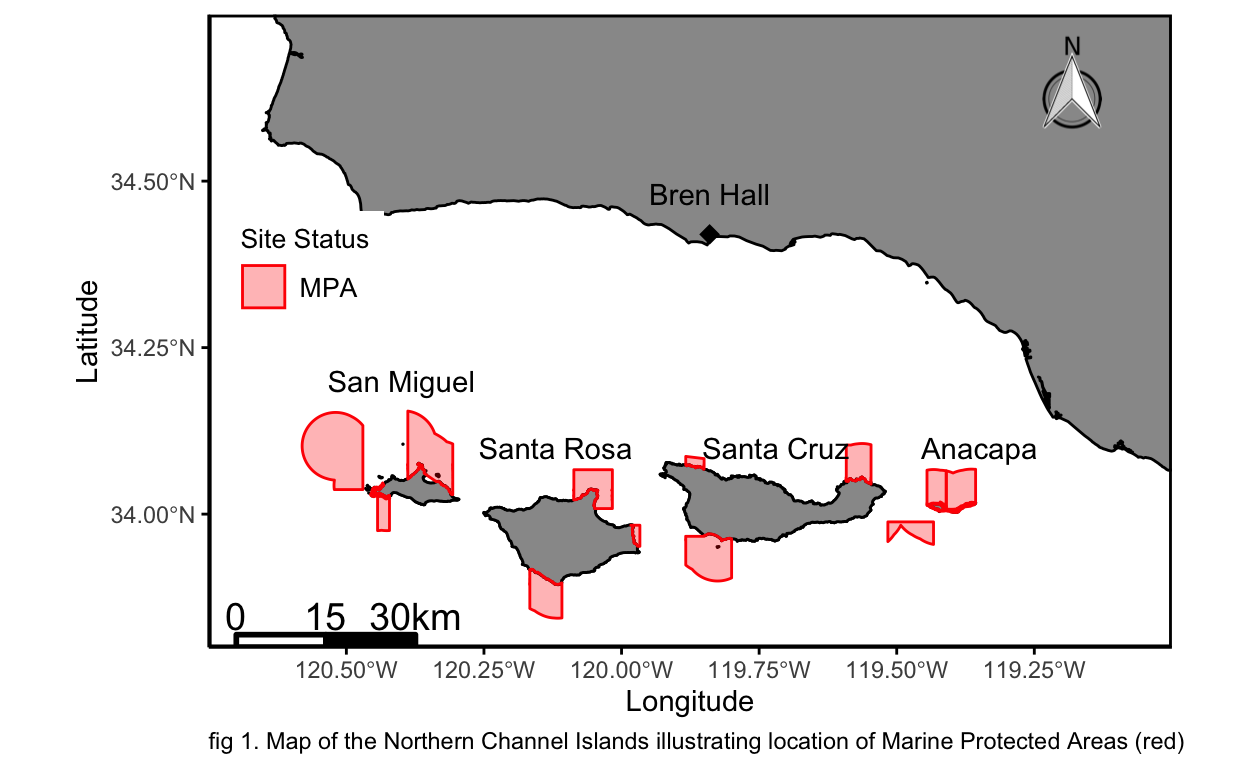
\includegraphics{mpasandkelp_files/figure-latex/unnamed-chunk-1-1.pdf}

An array work has already been done analyzing the effects of MPA
implementation on Kelp Forests (Hamilton \& Caselle, 2015, Selden et
al.~2017). It is well known that many trophic levels change in abundance
whether in an MPA or in a fished area (A Decade of Protection, PISCO).
It is also well know that Purple urchins can form ``barrens'' when
densities reach a critical threshold (Ling et al., 2015). There is a
tipping point where a phase-shift occurs from a macro-algae dominated
system to an urchin barren (Dexter \& Scheibling, 2014). The reef will
become completely devoid of algae and the dominate space holder will be
purple urchins(Ling et al., 2015, Dexter \& Scheibling, 2014).

I began conducting sub-tidal surveys for PISCO in 2017 and have
developed these questions based on anecdotal evidence. It was always
visually evident if we were surveying in an MPA or reference site based
on kelp and urchin densities. MPAs visually had more kelp and less
urchins while reference sites visually had less kelp and more urchins.

In this study I will test my anecdotal questions with PISCO data. I ask
the question; Do MPAs increase kelp densities and what invertebrate
species inhibit kelp densities? I also take a simplistic approach and
address the question; At what point do MPAs and reference sites kelp
densities significantly differ following MPA implementation?

\hypertarget{methods}{%
\subsubsection{Methods}\label{methods}}

In order to answer the desired questions I have obtained PISCO data
running from 1999 to 2020. I have chosen to look at Anacapa Island,
Santa Cruz Island, Santa Rosa Island, and San Miguel Island as those
islands are the predominant data source for PISCO N. Channel Island
survey sites (fig 1).

Data was collected through annual sub-tidal scuba surveys. 12 benthic
transects (30 x 2 x 2 m) are surveyed at each site between June and
August to quantify densities of invertebrates and macro-algae. Benthic
surveys are stratified into three depth zones (approximately 5-, 10-,
and 15-m depth). Giant kelp (Macrocystis pyrifera) (kelp) individuals
greater than 1-m in height are counted and stipes are enumerated per
individual and later summed at the transect level for analysis. Purple
urchins (Strongylocentrotus purpuratus) greater than 2.5 cm in diameter
are counted. Sites are either categorized as MPAs or reference sites,
each MPA has a paired reference site.

Data was averaged to an annual site mean (n=658, MPA: n=310, Reference:
n=348) for purple urchins and kelp stipes (kelp). Understory kelps and
red urchins were not included as Giant kelp is the predominant
structural species and red urchins are commercially fished.

All analysis was conducted in Rstudio and the code repository is linked
(see supporting figures). OLS linear models and whelch two sample t
tests (\(\alpha\) \textless{} 0.05) were conducted based on previous
studies understandings of affects purple urchins can have on kelp
densities when urchin populations are left unchecked. Response variables
were log transformed in order to normalize distribution (see supporting
figures). The QQplot is not linear and the residuals show potential
heteroscedasticity, model results should guide further research (see
supporting figures). All other tests of model fit did show potential for
acceptable model choice.

\begin{Shaded}
\begin{Highlighting}[]
\NormalTok{raw\_data }\OtherTok{\textless{}{-}} \FunctionTok{read\_csv}\NormalTok{(}\FunctionTok{here}\NormalTok{(}\StringTok{"\_posts"}\NormalTok{, }\StringTok{"2021{-}11{-}29{-}mpasandkelp"}\NormalTok{, }\StringTok{"MLPA\_swath\_site\_means.csv"}\NormalTok{))}


\NormalTok{annual\_mean }\OtherTok{\textless{}{-}}\NormalTok{ raw\_data }\SpecialCharTok{\%\textgreater{}\%} 
  \FunctionTok{filter}\NormalTok{(campus }\SpecialCharTok{==} \StringTok{"UCSB"}\NormalTok{) }\SpecialCharTok{\%\textgreater{}\%}
  \FunctionTok{separate}\NormalTok{(}\AttributeTok{col =}\NormalTok{ site, }\AttributeTok{into =} \FunctionTok{c}\NormalTok{(}\StringTok{\textquotesingle{}island\textquotesingle{}}\NormalTok{, }\StringTok{\textquotesingle{}site\textquotesingle{}}\NormalTok{), }\AttributeTok{sep =} \StringTok{\textquotesingle{}\_\textquotesingle{}}\NormalTok{) }\SpecialCharTok{\%\textgreater{}\%} 
  \FunctionTok{filter}\NormalTok{(island }\SpecialCharTok{\%in\%} \FunctionTok{c}\NormalTok{(}\StringTok{"ANACAPA"}\NormalTok{, }\StringTok{"SCI"}\NormalTok{, }\StringTok{"SRI"}\NormalTok{, }\StringTok{"SMI"}\NormalTok{)) }\SpecialCharTok{\%\textgreater{}\%} 
  \FunctionTok{select}\NormalTok{(}\FunctionTok{c}\NormalTok{(}\StringTok{"survey\_year"}\NormalTok{, }\StringTok{"site"}\NormalTok{, }\StringTok{"island"}\NormalTok{, }\StringTok{"latitude"}\NormalTok{, }
           \StringTok{"longitude"}\NormalTok{, }\StringTok{"site\_status"}\NormalTok{,}
           \StringTok{"den\_STRPURAD"}\NormalTok{, }\StringTok{"den\_MACPYRAD"}\NormalTok{, }\StringTok{"den\_MACSTIPES"}\NormalTok{)) }\SpecialCharTok{\%\textgreater{}\%} 
  \FunctionTok{group\_by}\NormalTok{(survey\_year, site\_status) }\SpecialCharTok{\%\textgreater{}\%} 
  \FunctionTok{mutate}\NormalTok{(}\AttributeTok{mean\_purp =} \FunctionTok{mean}\NormalTok{(den\_STRPURAD),}
         \AttributeTok{mean\_stipe =} \FunctionTok{mean}\NormalTok{(den\_MACSTIPES),}
         \AttributeTok{mean\_mac =} \FunctionTok{mean}\NormalTok{(den\_MACPYRAD)) }\SpecialCharTok{\%\textgreater{}\%} 
  \FunctionTok{mutate}\NormalTok{(}\AttributeTok{log\_urch =} \FunctionTok{log}\NormalTok{(den\_STRPURAD)) }\SpecialCharTok{\%\textgreater{}\%} 
  \FunctionTok{mutate}\NormalTok{(}\AttributeTok{log\_mac =} \FunctionTok{log}\NormalTok{(den\_MACSTIPES)) }\SpecialCharTok{\%\textgreater{}\%}
  \FunctionTok{mutate}\NormalTok{(}\AttributeTok{log\_plant =} \FunctionTok{log}\NormalTok{(den\_MACPYRAD)) }\SpecialCharTok{\%\textgreater{}\%} 
  \FunctionTok{filter\_all}\NormalTok{(}\FunctionTok{all\_vars}\NormalTok{(}\SpecialCharTok{!}\FunctionTok{is.infinite}\NormalTok{(.))) }\SpecialCharTok{\%\textgreater{}\%} 
  \FunctionTok{ungroup}\NormalTok{()}
\end{Highlighting}
\end{Shaded}

\hypertarget{results}{%
\subsubsection{Results}\label{results}}

Through initial data visualization, trends can be observed for kelp
densities and urchin densities inside MPAs and reference sites (fig 2).
It is apparent that urchin densities between MPAs and reference sites
fluctuate and follow similar trends until 2014, in which urchin
densities inside MPAs show considerably lower densities. A similar trend
is observed for kelp densities in which densities fluctuate until 2013
and then began to diverge with higher densities inside the MPAs.

\begin{Shaded}
\begin{Highlighting}[]
\NormalTok{urchins }\OtherTok{\textless{}{-}} \FunctionTok{ggplot}\NormalTok{(}\AttributeTok{data =}\NormalTok{ annual\_mean) }\SpecialCharTok{+}
  \FunctionTok{geom\_line}\NormalTok{(}\FunctionTok{aes}\NormalTok{(}\AttributeTok{x =}\NormalTok{ survey\_year, }\AttributeTok{y =}\NormalTok{ mean\_purp, }\AttributeTok{color =}\NormalTok{ site\_status)) }\SpecialCharTok{+}
  \FunctionTok{theme\_classic}\NormalTok{() }\SpecialCharTok{+}
  \FunctionTok{xlab}\NormalTok{(}\StringTok{"Year"}\NormalTok{)}\SpecialCharTok{+}
  \FunctionTok{ylab}\NormalTok{(}\FunctionTok{expression}\NormalTok{(}\StringTok{"Urchin Density per 60m"}\SpecialCharTok{\^{}}\DecValTok{2}\NormalTok{)) }\SpecialCharTok{+}
  \FunctionTok{labs}\NormalTok{(}\AttributeTok{color =} \StringTok{"Site Status"}\NormalTok{) }\SpecialCharTok{+}
  \FunctionTok{scale\_color\_manual}\NormalTok{(}\AttributeTok{values =} \FunctionTok{c}\NormalTok{(}\StringTok{"red"}\NormalTok{, }\StringTok{"blue"}\NormalTok{)) }\SpecialCharTok{+}
  \FunctionTok{labs}\NormalTok{(}\AttributeTok{title =} \StringTok{"Northern Channel Islands"}\NormalTok{) }\SpecialCharTok{+}
  \FunctionTok{theme}\NormalTok{(}\AttributeTok{plot.title =} \FunctionTok{element\_text}\NormalTok{(}\AttributeTok{hjust =} \FloatTok{0.5}\NormalTok{))}




\NormalTok{kelp }\OtherTok{\textless{}{-}} \FunctionTok{ggplot}\NormalTok{(}\AttributeTok{data =}\NormalTok{ annual\_mean) }\SpecialCharTok{+}
  \FunctionTok{geom\_line}\NormalTok{(}\FunctionTok{aes}\NormalTok{(}\AttributeTok{x =}\NormalTok{ survey\_year, }\AttributeTok{y =}\NormalTok{ mean\_stipe, }\AttributeTok{color =}\NormalTok{ site\_status), }\AttributeTok{show.legend =}\NormalTok{ F) }\SpecialCharTok{+}
  \FunctionTok{theme\_classic}\NormalTok{()}\SpecialCharTok{+}
  \FunctionTok{xlab}\NormalTok{(}\StringTok{"Year"}\NormalTok{)}\SpecialCharTok{+}
  \FunctionTok{ylab}\NormalTok{(}\FunctionTok{expression}\NormalTok{(}\StringTok{"Kelp Density per 60m"}\SpecialCharTok{\^{}}\DecValTok{2}\NormalTok{)) }\SpecialCharTok{+}
  \FunctionTok{labs}\NormalTok{(}\AttributeTok{color =} \StringTok{"Site Status"}\NormalTok{)  }\SpecialCharTok{+}
  \FunctionTok{scale\_color\_manual}\NormalTok{(}\AttributeTok{values =} \FunctionTok{c}\NormalTok{(}\StringTok{"red"}\NormalTok{, }\StringTok{"blue"}\NormalTok{)) }\SpecialCharTok{+} 
  \FunctionTok{labs}\NormalTok{(}\AttributeTok{caption =} \StringTok{"fig 2. Change in Purple Urchin and Kelp Densities in MPAs and Reference sites at the N. Channel Islands"}\NormalTok{) }\SpecialCharTok{+}
  \FunctionTok{theme}\NormalTok{(}\AttributeTok{plot.caption =} \FunctionTok{element\_text}\NormalTok{(}\AttributeTok{hjust =} \DecValTok{0}\NormalTok{))}

  


\NormalTok{combined }\OtherTok{\textless{}{-}}\NormalTok{ urchins }\SpecialCharTok{/}\NormalTok{ kelp }\SpecialCharTok{\&} \FunctionTok{theme}\NormalTok{(}\AttributeTok{legend.position =} \StringTok{"right"}\NormalTok{) }
\NormalTok{combined }\SpecialCharTok{+} \FunctionTok{plot\_layout}\NormalTok{(}\AttributeTok{guides =} \StringTok{"collect"}\NormalTok{)}
\end{Highlighting}
\end{Shaded}

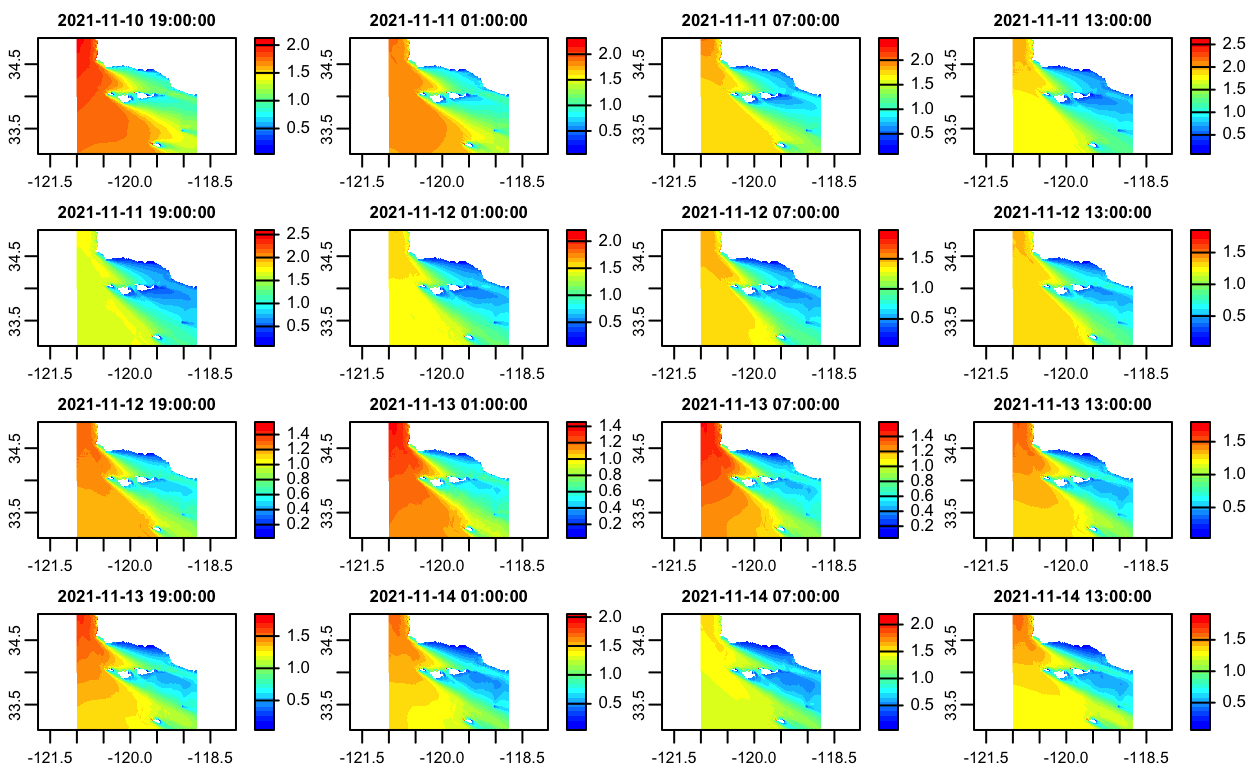
\includegraphics{mpasandkelp_files/figure-latex/unnamed-chunk-3-1.pdf}

\hypertarget{linear-model}{%
\paragraph{Linear Model}\label{linear-model}}

To determine what might be the cause of these differences of kelp
densities in the MPAs and reference sites, a linear model was created
(\(\alpha\) \textless{} 0.05) (Tbl 1, fig 3). Annual site means for
urchin densities, site status (MPA or Reference Site), and site status
as an interaction with urchin densities, were all used as predictors for
log kelp densities in the linear model. The results illustrate that
urchin density is a significant predictor for log kelp densities
(p\textless0.001). Interestingly site status is a poor predictor for log
kelp densities (p=0.845) yet anecdotal observations say otherwise. The
urchin density and site status interaction (p=0.095) was not found to be
a significant interaction but can still indicate the affects that can
occur between the two predictors. A negative trend can clearly be seen
between log kelp density and urchin densities (fig 3). Overall model
predictability is rather low (adjusted \(R^{2}\) = 0.154) and not suited
for predicting log kelp variability.

\begin{Shaded}
\begin{Highlighting}[]
\NormalTok{mod }\OtherTok{\textless{}{-}} \FunctionTok{lm}\NormalTok{(log\_mac }\SpecialCharTok{\textasciitilde{}}\NormalTok{ den\_STRPURAD }\SpecialCharTok{+}\NormalTok{ site\_status }\SpecialCharTok{+}\NormalTok{ site\_status}\SpecialCharTok{:}\NormalTok{den\_STRPURAD, }
        \AttributeTok{data =}\NormalTok{ annual\_mean)}

\FunctionTok{tab\_model}\NormalTok{(mod,}
          \AttributeTok{pred.labels =} \FunctionTok{c}\NormalTok{(}\StringTok{"Intercept"}\NormalTok{, }\StringTok{"Urchin Density"}\NormalTok{, }\StringTok{"Site Status"}\NormalTok{, }
                          \StringTok{"Urchin Density:Site Status"}\NormalTok{),}
          \AttributeTok{dv.labels =} \FunctionTok{c}\NormalTok{(}\StringTok{"log Kelp Density"}\NormalTok{),}
          \AttributeTok{string.ci =} \StringTok{"Conf. Int (95\%)"}\NormalTok{,}
          \AttributeTok{string.p =} \StringTok{"P{-}value"}\NormalTok{,}
          \AttributeTok{title =} \StringTok{"Tbl 1. Linear Model Results for Below Predictors"}\NormalTok{)}
\end{Highlighting}
\end{Shaded}

Tbl 1. Linear Model Results for Below Predictors

~

log Kelp Density

Predictors

Estimates

Conf. Int (95\%)

P-value

Intercept

5.01

4.81~--~5.21

\textless0.001

Urchin Density

-0.00

-0.00~--~-0.00

\textless0.001

Site Status

0.03

-0.25~--~0.31

0.845

Urchin Density:Site Status

0.00

-0.00~--~0.00

0.095

Observations

658

R2 / R2 adjusted

0.158 / 0.154

\begin{Shaded}
\begin{Highlighting}[]
\NormalTok{annual\_mean }\SpecialCharTok{\%\textgreater{}\%} 
  \FunctionTok{ggplot}\NormalTok{(}\FunctionTok{aes}\NormalTok{(}\AttributeTok{x =}\NormalTok{ den\_STRPURAD, }\AttributeTok{y =}\NormalTok{ log\_mac, }\AttributeTok{color =}\NormalTok{ site\_status)) }\SpecialCharTok{+}
  \FunctionTok{geom\_point}\NormalTok{(}\AttributeTok{alpha =} \FloatTok{0.5}\NormalTok{, }\FunctionTok{aes}\NormalTok{(}\AttributeTok{color =}\NormalTok{site\_status)) }\SpecialCharTok{+}
  \FunctionTok{geom\_smooth}\NormalTok{(}\AttributeTok{formula =}\NormalTok{ y }\SpecialCharTok{\textasciitilde{}}\NormalTok{ x, }\AttributeTok{method =} \StringTok{"lm"}\NormalTok{, }\AttributeTok{se =}\NormalTok{ T, }\AttributeTok{lwd =} \FloatTok{0.8}\NormalTok{) }\SpecialCharTok{+}
  \FunctionTok{theme\_classic}\NormalTok{() }\SpecialCharTok{+}
  \FunctionTok{scale\_y\_continuous}\NormalTok{(}\AttributeTok{expand =} \FunctionTok{c}\NormalTok{(}\FloatTok{0.01}\NormalTok{,}\FloatTok{0.01}\NormalTok{)) }\SpecialCharTok{+}
  \FunctionTok{scale\_x\_continuous}\NormalTok{(}\AttributeTok{expand =} \FunctionTok{c}\NormalTok{(}\FloatTok{0.01}\NormalTok{,}\FloatTok{0.01}\NormalTok{)) }\SpecialCharTok{+}
  \FunctionTok{ylab}\NormalTok{(}\FunctionTok{expression}\NormalTok{(}\StringTok{"log Kelp Density per 60m"}\SpecialCharTok{\^{}}\DecValTok{2}\NormalTok{)) }\SpecialCharTok{+}
  \FunctionTok{xlab}\NormalTok{(}\FunctionTok{expression}\NormalTok{(}\StringTok{"Urchin Density per 60m"}\SpecialCharTok{\^{}}\DecValTok{2}\NormalTok{)) }\SpecialCharTok{+}
  \FunctionTok{labs}\NormalTok{(}\AttributeTok{color =} \StringTok{"Site Status"}\NormalTok{,}
       \AttributeTok{caption =} \StringTok{"fig 3. Linear model of Urchin Density, Site Status, and Site Status:Urchin Density as predictors of log Kelp"}\NormalTok{) }\SpecialCharTok{+}
  \FunctionTok{scale\_color\_manual}\NormalTok{(}\AttributeTok{values =} \FunctionTok{c}\NormalTok{(}\StringTok{"red"}\NormalTok{, }\StringTok{"blue"}\NormalTok{))}
\end{Highlighting}
\end{Shaded}

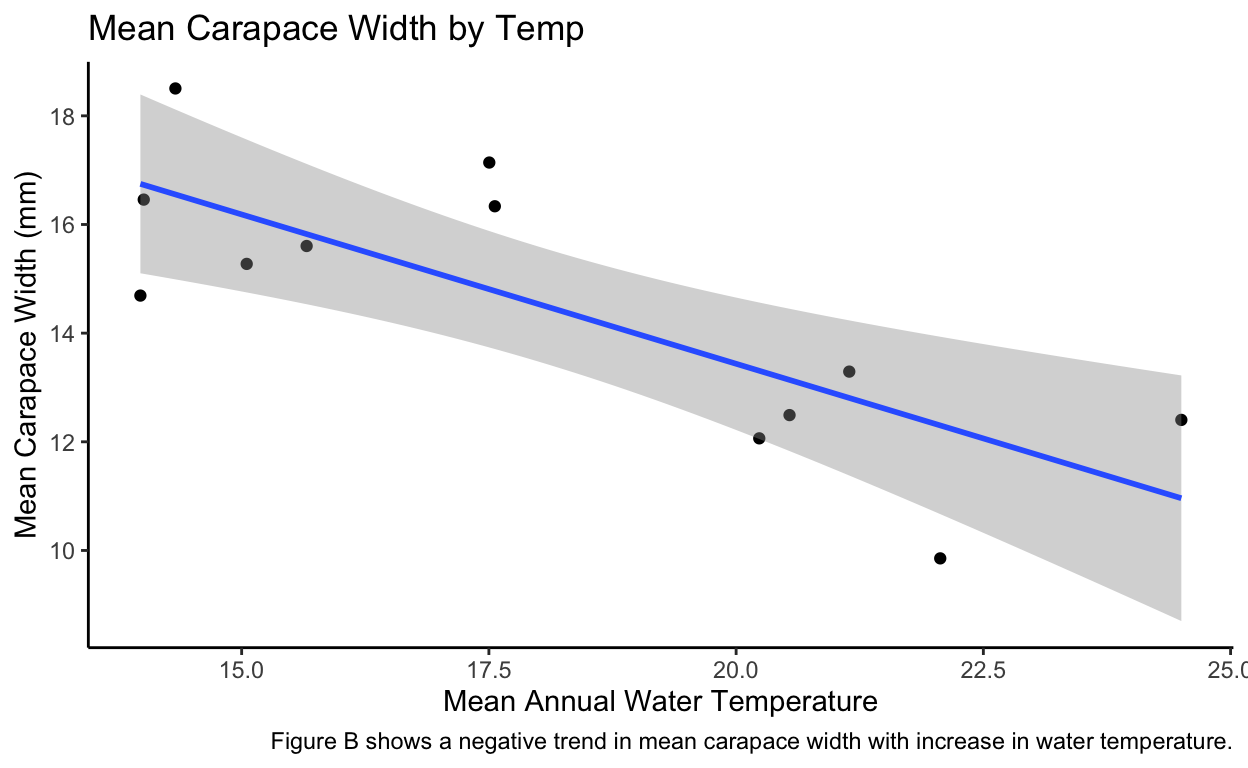
\includegraphics{mpasandkelp_files/figure-latex/unnamed-chunk-4-1.pdf}

\hypertarget{welch-two-sample-t-test}{%
\paragraph{Welch Two Sample T Test}\label{welch-two-sample-t-test}}

In order to test my anecdotal evidence of higher densities of kelp and
lower densities of urchins in the MPAs and vice versa for reference
sites, I have created a set of Welch Two Sample t-tests (\(\alpha\)
\textless{} 0.05).

The null hypothesis: There is no difference of kelp and urchin densities
between MPAs and reference sites for the selected data set.

The alternative hypothesis: There is a difference in kelp and urchin
densities between MPAs and reference sites for the selected data set.

The first t-test concluded that we would fail to reject the null
hypothesis of site status as a predictor for log kelp density (p=0.675)
(fig 3 Tbl 2). The second t-test once again concluded that we would fail
to reject the null hypothesis of site status as a predictor for log
urchin density (p=0.846) (fig 4 Tbl 3). This may not align with my
current anecdotal evidence and that is understandable as these t-tests
include many data points through time that counter my current anecdotal
evidence (fig 2).

\begin{Shaded}
\begin{Highlighting}[]
\CommentTok{\#null: no difference of kelp and urchins across reference sites and mpas}

\CommentTok{\#alternative: there is a difference}


\NormalTok{kelp.test }\OtherTok{\textless{}{-}}\FunctionTok{t.test}\NormalTok{(log\_mac }\SpecialCharTok{\textasciitilde{}}\NormalTok{ site\_status, }\AttributeTok{data =}\NormalTok{ annual\_mean)}


\FunctionTok{tab\_model}\NormalTok{(kelp.test,}
          \AttributeTok{string.ci =} \FunctionTok{c}\NormalTok{(}\StringTok{"Conf. Int (95\%)"}\NormalTok{),}
          \AttributeTok{string.p =} \StringTok{"P{-}value"}\NormalTok{,}
          \AttributeTok{dv.labels =} \FunctionTok{c}\NormalTok{(}\StringTok{"log Kelp Density"}\NormalTok{),}
          \AttributeTok{pred.labels =} \StringTok{"Site Status"}\NormalTok{,}
          \AttributeTok{title =} \StringTok{"Tbl 2. log Kelp Welch Two Sample t{-}test"}\NormalTok{)}
\end{Highlighting}
\end{Shaded}

Tbl 2. log Kelp Welch Two Sample t-test

~

log Kelp Density

Predictors

Estimates

Conf. Int (95\%)

P-value

Site Status

-0.05

-0.30~--~0.19

0.675

\begin{Shaded}
\begin{Highlighting}[]
\NormalTok{kelp\_boxp }\OtherTok{\textless{}{-}} \FunctionTok{ggboxplot}\NormalTok{(annual\_mean, }\AttributeTok{x =} \StringTok{"site\_status"}\NormalTok{, }\AttributeTok{y =} \StringTok{"log\_mac"}\NormalTok{,}
                     \AttributeTok{xlab =} \StringTok{"Site Status"}\NormalTok{, }\AttributeTok{ylab =} \FunctionTok{expression}\NormalTok{(}\StringTok{"log Kelp Density per 60m"}\SpecialCharTok{\^{}}\DecValTok{2}\NormalTok{), }
                     \AttributeTok{title =} \StringTok{"fig 3. T Test, t(616.94) = 2.5502, p = 0.7993, n = 658"}\NormalTok{,}
                     \AttributeTok{bxp.errorbar =}\NormalTok{ T,}
                     \AttributeTok{alpha =} \FloatTok{0.3}\NormalTok{, }
                     \AttributeTok{color =} \FunctionTok{c}\NormalTok{(}\StringTok{"blue"}\NormalTok{, }\StringTok{"red"}\NormalTok{))}

\NormalTok{kelp\_boxp}
\end{Highlighting}
\end{Shaded}

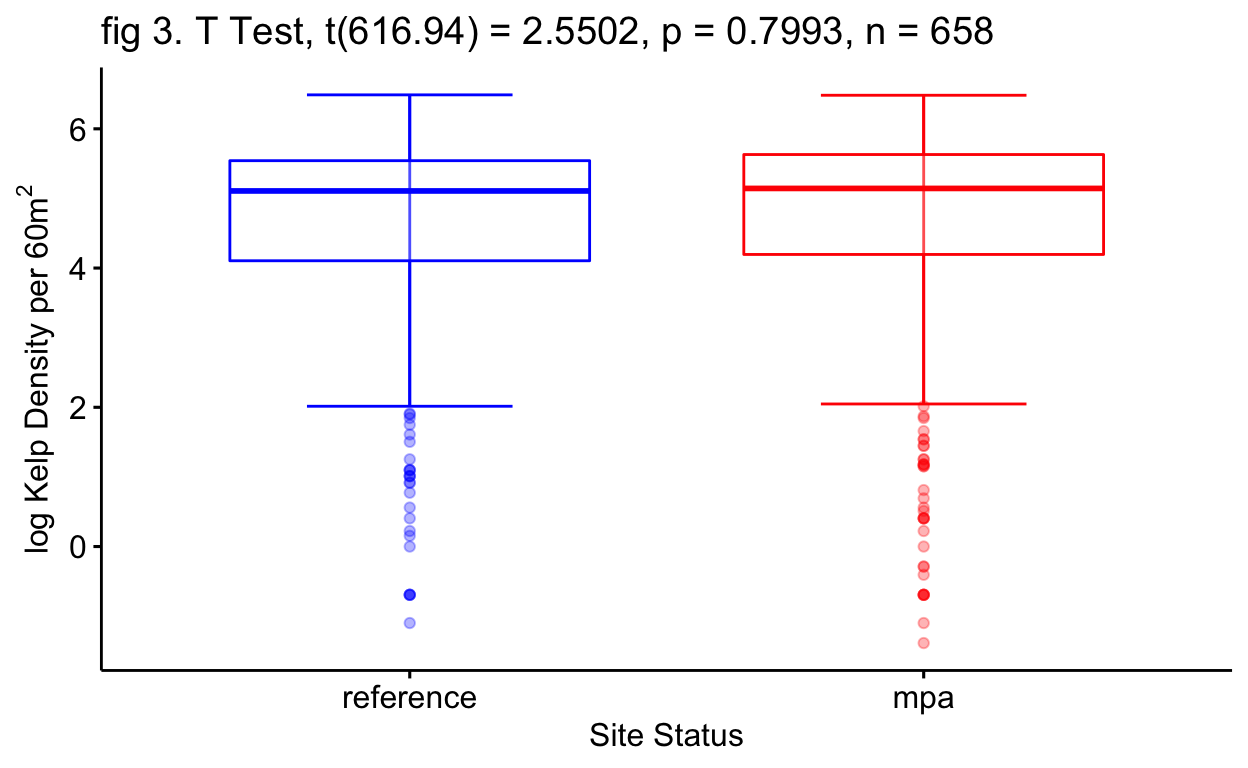
\includegraphics{mpasandkelp_files/figure-latex/unnamed-chunk-5-1.pdf}

\begin{Shaded}
\begin{Highlighting}[]
\NormalTok{urch }\OtherTok{\textless{}{-}} \FunctionTok{t.test}\NormalTok{(log\_urch }\SpecialCharTok{\textasciitilde{}}\NormalTok{ site\_status , }\AttributeTok{data =}\NormalTok{ annual\_mean)}

\FunctionTok{tab\_model}\NormalTok{(urch,}
          \AttributeTok{string.ci =} \StringTok{"Conf. Int (95\%)"}\NormalTok{,}
          \AttributeTok{string.p =} \StringTok{"P{-}value"}\NormalTok{,}
          \AttributeTok{dv.labels =} \StringTok{"log Urchin Density"}\NormalTok{,}
          \AttributeTok{pred.labels =} \StringTok{"Site Status"}\NormalTok{,}
          \AttributeTok{title =} \StringTok{"Tbl 3. log Urchin Welch Two Sample t{-}test"}\NormalTok{)}
\end{Highlighting}
\end{Shaded}

Tbl 3. log Urchin Welch Two Sample t-test

~

log Urchin Density

Predictors

Estimates

Conf. Int (95\%)

P-value

Site Status

-0.03

-0.34~--~0.28

0.846

\begin{Shaded}
\begin{Highlighting}[]
\NormalTok{urch\_bxp }\OtherTok{\textless{}{-}}\FunctionTok{ggboxplot}\NormalTok{(annual\_mean, }\AttributeTok{x =} \StringTok{"site\_status"}\NormalTok{, }\AttributeTok{y =} \StringTok{"log\_urch"}\NormalTok{,}
                     \AttributeTok{xlab =} \StringTok{"Site Status"}\NormalTok{, }\AttributeTok{ylab =} \FunctionTok{expression}\NormalTok{(}\StringTok{"log Urchin Density per 60m"}\SpecialCharTok{\^{}}\DecValTok{2}\NormalTok{), }
                     \AttributeTok{title =} \StringTok{"fig 4. T Test, t(647.41) = {-}0.19433, p = 0.846, n = 658"}\NormalTok{,}
                     \AttributeTok{bxp.errorbar =}\NormalTok{ T,}
                     \AttributeTok{alpha =} \FloatTok{0.3}\NormalTok{, }
                     \AttributeTok{color =} \FunctionTok{c}\NormalTok{(}\StringTok{"blue"}\NormalTok{, }\StringTok{"red"}\NormalTok{))}



\NormalTok{urch\_bxp}
\end{Highlighting}
\end{Shaded}

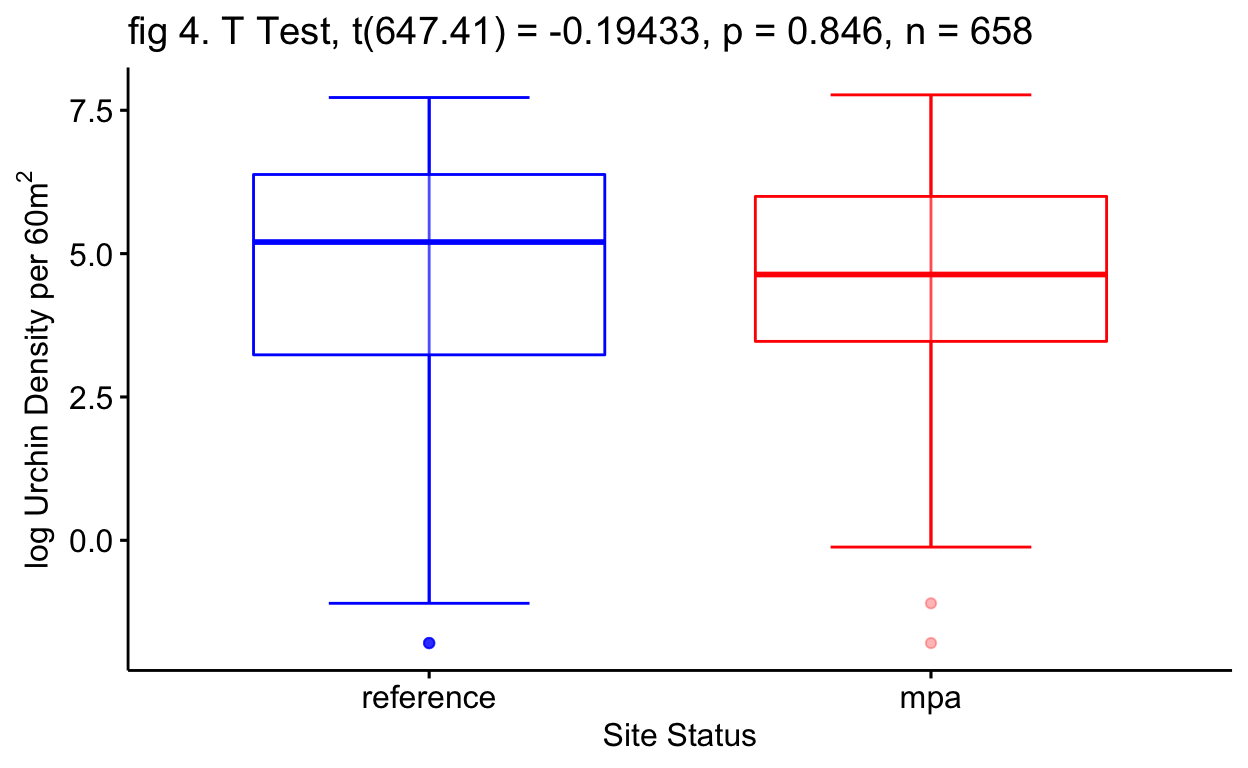
\includegraphics{mpasandkelp_files/figure-latex/unnamed-chunk-5-2.pdf}

\hypertarget{mpa-implementation-linear-model}{%
\paragraph{MPA Implementation Linear
Model}\label{mpa-implementation-linear-model}}

In order to test the affects of time since MPA implementation on kelp
densities both in MPAs and reference sites a linear model was created
with time since MPA implementation as a predictor for log kelp densities
(Tbl 4 \& 5). A significant difference (\(\alpha\) \textless{} 0.05) in
kelp densities since the implementation of the MPAs occurred for years
15-18 (p=0.019, 0.012, 0.008, 0.01) after implementation or 2017-2020
(fig 6 Tbl 4).

A similar trend occurred for the reference sites. A significant
difference in kelp densities since the implementation of MPAs occurred
12, 14-17 (p=0.001, \textless0.001, \textless0.001, 0.002,
\textless0.001) years after implementation or 2014, 2016, 2017-2019.

\begin{Shaded}
\begin{Highlighting}[]
\NormalTok{time\_lag\_mpa }\OtherTok{\textless{}{-}}\NormalTok{ annual\_mean }\SpecialCharTok{\%\textgreater{}\%} 
  \FunctionTok{filter}\NormalTok{(site\_status }\SpecialCharTok{==} \StringTok{"mpa"}\NormalTok{,}
\NormalTok{         survey\_year }\SpecialCharTok{\textgreater{}}\DecValTok{2000}\NormalTok{)}\SpecialCharTok{\%\textgreater{}\%}
  \FunctionTok{group\_by}\NormalTok{(survey\_year) }\SpecialCharTok{\%\textgreater{}\%} 
  \FunctionTok{add\_column}\NormalTok{(}\AttributeTok{time\_mpa =} \StringTok{""}\NormalTok{)}

\NormalTok{time\_lag\_mpa}\SpecialCharTok{$}\NormalTok{time\_mpa }\OtherTok{\textless{}{-}} \FunctionTok{cut}\NormalTok{(time\_lag\_mpa}\SpecialCharTok{$}\NormalTok{survey\_year, }
                             \FunctionTok{c}\NormalTok{(}\DecValTok{2002}\SpecialCharTok{:}\DecValTok{2020}\NormalTok{), }\FunctionTok{c}\NormalTok{(}\DecValTok{1}\SpecialCharTok{:}\DecValTok{18}\NormalTok{))}

\NormalTok{time\_lag\_mpa }\OtherTok{\textless{}{-}}\NormalTok{ time\_lag\_mpa }\SpecialCharTok{\%\textgreater{}\%}
   \FunctionTok{filter}\NormalTok{(survey\_year }\SpecialCharTok{\textgreater{}} \DecValTok{2002}\NormalTok{)}



\NormalTok{mpa\_mod }\OtherTok{\textless{}{-}} \FunctionTok{lm}\NormalTok{(log\_mac }\SpecialCharTok{\textasciitilde{}}\NormalTok{ time\_mpa, }
              \AttributeTok{data =}\NormalTok{ time\_lag\_mpa)}

\FunctionTok{tab\_model}\NormalTok{(mpa\_mod, }\AttributeTok{df.method =} \StringTok{"kr"}\NormalTok{,}
          \AttributeTok{string.ci =} \StringTok{"Conf. Int (95\%)"}\NormalTok{,}
          \AttributeTok{string.p =} \StringTok{"P{-}value"}\NormalTok{,}
          \AttributeTok{pred.labels =} \FunctionTok{c}\NormalTok{(}\StringTok{"Intercept"}\NormalTok{, }\StringTok{"2 Years"}\NormalTok{, }\StringTok{"3 Years"}\NormalTok{, }\StringTok{"4 Years"}\NormalTok{, }\StringTok{"5 Years"}\NormalTok{, }\StringTok{"6 Years"}\NormalTok{,}
                          \StringTok{"7 Years"}\NormalTok{, }\StringTok{"8 Years"}\NormalTok{, }\StringTok{"9 Years"}\NormalTok{, }\StringTok{"10 Years"}\NormalTok{, }\StringTok{"11 Years"}\NormalTok{, }\StringTok{"12 Years"}\NormalTok{, }\StringTok{"13 Years"}\NormalTok{, }\StringTok{"14 Years"}\NormalTok{,}
                          \StringTok{"15 Years"}\NormalTok{, }\StringTok{"16 Years"}\NormalTok{, }\StringTok{"17 Years"}\NormalTok{, }\StringTok{"18 Years"}\NormalTok{),}
          \AttributeTok{dv.labels =} \FunctionTok{c}\NormalTok{(}\StringTok{"log Kelp Density"}\NormalTok{),}
          \AttributeTok{title =} \StringTok{"Tbl 4 Linear model fit for change in MPA kelp density since implementation"}\NormalTok{)}
\end{Highlighting}
\end{Shaded}

Tbl 4 Linear model fit for change in MPA kelp density since
implementation

~

log Kelp Density

Predictors

Estimates

Conf. Int (95\%)

P-value

Intercept

3.86

2.90~--~4.81

\textless0.001

2 Years

0.22

-1.13~--~1.56

0.751

3 Years

0.39

-0.83~--~1.60

0.532

4 Years

0.77

-0.57~--~2.12

0.259

5 Years

0.78

-0.40~--~1.96

0.195

6 Years

0.23

-0.96~--~1.42

0.707

7 Years

0.23

-0.92~--~1.39

0.690

8 Years

0.88

-0.37~--~2.12

0.166

9 Years

-0.06

-1.33~--~1.22

0.931

10 Years

0.36

-0.93~--~1.66

0.583

11 Years

0.45

-0.92~--~1.83

0.518

12 Years

0.25

-0.98~--~1.48

0.691

13 Years

0.88

-0.37~--~2.14

0.168

14 Years

-0.26

-1.52~--~0.99

0.680

15 Years

1.49

0.25~--~2.73

0.019

16 Years

1.60

0.36~--~2.84

0.012

17 Years

1.71

0.45~--~2.96

0.008

18 Years

1.67

0.41~--~2.92

0.010

Observations

296

R2 / R2 adjusted

0.120 / 0.066

\begin{Shaded}
\begin{Highlighting}[]
\NormalTok{time\_lag\_ref }\OtherTok{\textless{}{-}}\NormalTok{ annual\_mean }\SpecialCharTok{\%\textgreater{}\%} 
  \FunctionTok{filter}\NormalTok{(site\_status }\SpecialCharTok{==} \StringTok{"reference"}\NormalTok{,}
\NormalTok{         survey\_year }\SpecialCharTok{\textgreater{}}\DecValTok{2000}\NormalTok{)}\SpecialCharTok{\%\textgreater{}\%}
  \FunctionTok{group\_by}\NormalTok{(survey\_year) }\SpecialCharTok{\%\textgreater{}\%} 
  \FunctionTok{add\_column}\NormalTok{(}\AttributeTok{time\_ref =} \StringTok{""}\NormalTok{)}

\NormalTok{time\_lag\_ref}\SpecialCharTok{$}\NormalTok{time\_ref }\OtherTok{\textless{}{-}} \FunctionTok{cut}\NormalTok{(time\_lag\_ref}\SpecialCharTok{$}\NormalTok{survey\_year, }
                             \FunctionTok{c}\NormalTok{(}\DecValTok{2002}\SpecialCharTok{:}\DecValTok{2020}\NormalTok{), }\FunctionTok{c}\NormalTok{(}\DecValTok{1}\SpecialCharTok{:}\DecValTok{18}\NormalTok{))}

\NormalTok{time\_lag\_ref }\OtherTok{\textless{}{-}}\NormalTok{ time\_lag\_ref }\SpecialCharTok{\%\textgreater{}\%}
   \FunctionTok{filter}\NormalTok{(survey\_year }\SpecialCharTok{\textgreater{}} \DecValTok{2002}\NormalTok{)}

\NormalTok{ref\_mod }\OtherTok{\textless{}{-}} \FunctionTok{lm}\NormalTok{(log\_mac }\SpecialCharTok{\textasciitilde{}}\NormalTok{ time\_ref, }
              \AttributeTok{data =}\NormalTok{ time\_lag\_ref)}

\FunctionTok{tab\_model}\NormalTok{(ref\_mod, }\AttributeTok{df.method =} \StringTok{"kr"}\NormalTok{,}
          \AttributeTok{string.ci =} \StringTok{"Conf. Int (95\%)"}\NormalTok{,}
          \AttributeTok{string.p =} \StringTok{"P{-}value"}\NormalTok{,}
          \AttributeTok{pred.labels =} \FunctionTok{c}\NormalTok{(}\StringTok{"Intercept"}\NormalTok{, }\StringTok{"2 Years"}\NormalTok{, }\StringTok{"3 Years"}\NormalTok{, }\StringTok{"4 Years"}\NormalTok{, }\StringTok{"5 Years"}\NormalTok{, }\StringTok{"6 Years"}\NormalTok{,}
                          \StringTok{"7 Years"}\NormalTok{, }\StringTok{"8 Years"}\NormalTok{, }\StringTok{"9 Years"}\NormalTok{, }\StringTok{"10 Years"}\NormalTok{, }\StringTok{"12 Years"}\NormalTok{, }\StringTok{"13 Years"}\NormalTok{, }\StringTok{"14 Years"}\NormalTok{,}
                          \StringTok{"15 Years"}\NormalTok{, }\StringTok{"16 Years"}\NormalTok{, }\StringTok{"17 Years"}\NormalTok{, }\StringTok{"18 Years"}\NormalTok{),}
          \AttributeTok{dv.labels =} \FunctionTok{c}\NormalTok{(}\StringTok{"Reference Site: log Kelp Density"}\NormalTok{),}
          \AttributeTok{title =} \StringTok{"Tbl 5. Linear model fit for change in reference site kelp density since implementation"}\NormalTok{)}
\end{Highlighting}
\end{Shaded}

Tbl 5. Linear model fit for change in reference site kelp density since
implementation

~

Reference Site: log Kelp Density

Predictors

Estimates

Conf. Int (95\%)

P-value

Intercept

5.03

4.36~--~5.70

\textless0.001

2 Years

0.54

-0.34~--~1.43

0.228

3 Years

0.39

-0.48~--~1.26

0.377

4 Years

0.07

-0.82~--~0.95

0.880

5 Years

0.23

-0.58~--~1.03

0.577

6 Years

0.04

-0.77~--~0.85

0.929

7 Years

0.05

-0.75~--~0.85

0.907

8 Years

-0.21

-1.03~--~0.61

0.614

9 Years

-0.65

-1.48~--~0.19

0.127

10 Years

-0.34

-1.18~--~0.50

0.429

12 Years

-1.50

-2.39~--~-0.62

0.001

13 Years

-0.99

-1.99~--~0.00

0.051

14 Years

-2.23

-3.20~--~-1.26

\textless0.001

15 Years

-2.10

-3.05~--~-1.14

\textless0.001

16 Years

-1.47

-2.39~--~-0.55

0.002

17 Years

-1.71

-2.63~--~-0.78

\textless0.001

18 Years

-0.83

-1.80~--~0.14

0.094

Observations

332

R2 / R2 adjusted

0.303 / 0.267

\begin{Shaded}
\begin{Highlighting}[]
\NormalTok{kelp\_time\_mpa }\OtherTok{\textless{}{-}} \FunctionTok{ggplot}\NormalTok{(}\AttributeTok{data =}\NormalTok{ time\_lag\_mpa) }\SpecialCharTok{+}
  \FunctionTok{geom\_line}\NormalTok{(}\FunctionTok{aes}\NormalTok{(}\AttributeTok{x =}\NormalTok{ survey\_year, }\AttributeTok{y =}\NormalTok{ mean\_stipe), }\AttributeTok{color =} \StringTok{"darkgoldenrod"}\NormalTok{) }\SpecialCharTok{+}
  \FunctionTok{theme\_classic}\NormalTok{()}\SpecialCharTok{+}
  \FunctionTok{xlab}\NormalTok{(}\StringTok{"Year"}\NormalTok{)}\SpecialCharTok{+}
  \FunctionTok{ylab}\NormalTok{(}\FunctionTok{expression}\NormalTok{(}\StringTok{"Kelp Density per 60m"}\SpecialCharTok{\^{}}\DecValTok{2}\NormalTok{)) }\SpecialCharTok{+}
  \FunctionTok{labs}\NormalTok{(}\AttributeTok{color =} \StringTok{"Site Status"}\NormalTok{) }\SpecialCharTok{+}
  \FunctionTok{geom\_vline}\NormalTok{(}\AttributeTok{xintercept =} \DecValTok{2018}\NormalTok{, }\AttributeTok{linetype =} \StringTok{"dashed"}\NormalTok{)}\SpecialCharTok{+}
  \FunctionTok{geom\_vline}\NormalTok{(}\AttributeTok{xintercept =} \DecValTok{2019}\NormalTok{, }\AttributeTok{linetype =} \StringTok{"dashed"}\NormalTok{)}\SpecialCharTok{+}
  \FunctionTok{geom\_vline}\NormalTok{(}\AttributeTok{xintercept =} \DecValTok{2017}\NormalTok{, }\AttributeTok{linetype =} \StringTok{"dashed"}\NormalTok{) }\SpecialCharTok{+}
  \FunctionTok{geom\_vline}\NormalTok{(}\AttributeTok{xintercept =} \DecValTok{2020}\NormalTok{, }\AttributeTok{linetype =} \StringTok{"dashed"}\NormalTok{) }\SpecialCharTok{+}
  \FunctionTok{scale\_alpha\_continuous}\NormalTok{()}\SpecialCharTok{+}
  \FunctionTok{scale\_y\_continuous}\NormalTok{(}\AttributeTok{expand =} \FunctionTok{c}\NormalTok{(}\FloatTok{0.01}\NormalTok{,}\FloatTok{0.01}\NormalTok{)) }\SpecialCharTok{+}
  \FunctionTok{scale\_x\_continuous}\NormalTok{(}\AttributeTok{expand =} \FunctionTok{c}\NormalTok{(}\FloatTok{0.01}\NormalTok{,}\FloatTok{0.01}\NormalTok{)) }\SpecialCharTok{+}
  \FunctionTok{labs}\NormalTok{(}\AttributeTok{title =} \StringTok{"Time Since Implementation of Marine Protected Areas"}\NormalTok{, }\AttributeTok{subtitle =} \StringTok{"MPA"}\NormalTok{) }\SpecialCharTok{+}
  \FunctionTok{theme}\NormalTok{(}\AttributeTok{plot.title =} \FunctionTok{element\_text}\NormalTok{(}\AttributeTok{hjust =} \FloatTok{0.5}\NormalTok{))}


\NormalTok{kelp\_time\_ref }\OtherTok{\textless{}{-}} \FunctionTok{ggplot}\NormalTok{(}\AttributeTok{data =}\NormalTok{ time\_lag\_ref) }\SpecialCharTok{+}
  \FunctionTok{geom\_line}\NormalTok{(}\FunctionTok{aes}\NormalTok{(}\AttributeTok{x =}\NormalTok{ survey\_year, }\AttributeTok{y =}\NormalTok{ mean\_stipe), }
            \AttributeTok{color =} \StringTok{"darkgoldenrod"}\NormalTok{, }\AttributeTok{linetype =} \StringTok{"dashed"}\NormalTok{) }\SpecialCharTok{+}
  \FunctionTok{theme\_classic}\NormalTok{()}\SpecialCharTok{+}
  \FunctionTok{xlab}\NormalTok{(}\StringTok{"Year"}\NormalTok{)}\SpecialCharTok{+}
  \FunctionTok{ylab}\NormalTok{(}\FunctionTok{expression}\NormalTok{(}\StringTok{"Kelp Density per 60m"}\SpecialCharTok{\^{}}\DecValTok{2}\NormalTok{)) }\SpecialCharTok{+}
  \FunctionTok{labs}\NormalTok{(}\AttributeTok{color =} \StringTok{"Site Status"}\NormalTok{) }\SpecialCharTok{+}
  \FunctionTok{geom\_vline}\NormalTok{(}\AttributeTok{xintercept =} \DecValTok{2017}\NormalTok{, }\AttributeTok{linetype =} \StringTok{"dashed"}\NormalTok{)}\SpecialCharTok{+}
  \FunctionTok{geom\_vline}\NormalTok{(}\AttributeTok{xintercept =} \DecValTok{2018}\NormalTok{, }\AttributeTok{linetype =} \StringTok{"dashed"}\NormalTok{)}\SpecialCharTok{+}
  \FunctionTok{geom\_vline}\NormalTok{(}\AttributeTok{xintercept =} \DecValTok{2019}\NormalTok{, }\AttributeTok{linetype =} \StringTok{"dashed"}\NormalTok{) }\SpecialCharTok{+}
  \FunctionTok{geom\_vline}\NormalTok{(}\AttributeTok{xintercept =} \DecValTok{2016}\NormalTok{, }\AttributeTok{linetype =} \StringTok{"dashed"}\NormalTok{) }\SpecialCharTok{+}
  \FunctionTok{geom\_vline}\NormalTok{(}\AttributeTok{xintercept =} \DecValTok{2014}\NormalTok{, }\AttributeTok{linetype =} \StringTok{"dashed"}\NormalTok{) }\SpecialCharTok{+}
  \FunctionTok{scale\_y\_continuous}\NormalTok{(}\AttributeTok{expand =} \FunctionTok{c}\NormalTok{(}\FloatTok{0.01}\NormalTok{,}\FloatTok{0.01}\NormalTok{)) }\SpecialCharTok{+}
  \FunctionTok{scale\_x\_continuous}\NormalTok{(}\AttributeTok{expand =} \FunctionTok{c}\NormalTok{(}\FloatTok{0.01}\NormalTok{,}\FloatTok{0.01}\NormalTok{)) }\SpecialCharTok{+}
  \FunctionTok{labs}\NormalTok{(}\AttributeTok{subtitle =} \StringTok{"Reference Site"}\NormalTok{,}
       \AttributeTok{caption =} \StringTok{"fig 6. Change in kelp density indicating (dashed lines) years of significant (p\textless{}0.05) kelp differences since MPA implementation"}\NormalTok{) }

\NormalTok{kelp\_time\_mpa }\SpecialCharTok{/}\NormalTok{ kelp\_time\_ref}
\end{Highlighting}
\end{Shaded}

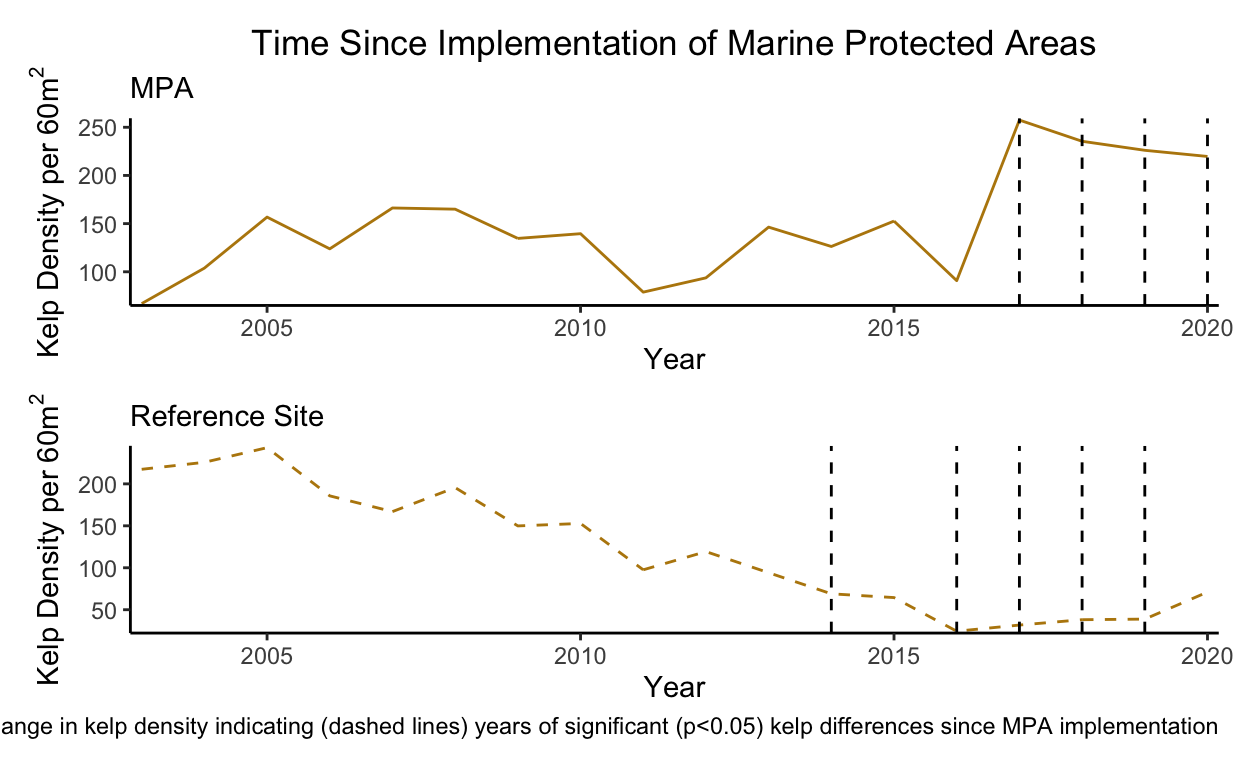
\includegraphics{mpasandkelp_files/figure-latex/unnamed-chunk-7-1.pdf}

\hypertarget{discussion}{%
\subsubsection{Discussion}\label{discussion}}

Understanding the changes that occur from the implementation of MPAs is
important so we can know if they are working and benefiting the
ecosystem. Through long term monitoring and analysis we can better
understand how they evolve through time and this knowledge can then be
translated across regions and systems for the implementation of new MPAs
or reserves.

From these results we can see changes in kelp densities from the
implementation of MPAs are not explicitly evident (fig 2). Kelp forests
are highly dynamic ecosystems and fluctuations caused through
environmental changes can lead to challenges in understanding changes
through time (fig 2) (Reed et al.~2014). However from our linear models
there does seem to be strong evidence of a negative relationship between
urchin densities and kelp densities (fig 3 Tbl 1). This significant
result (\(\alpha\) \textless{} 0.05) does line up with my own anecdotal
evidence of survey sites with high urchin densities and low kelp density
or vice versa. Interestingly, I did not see any evidence for site status
to significantlly affect either kelp or urchin densities (fig 3, 4, 5
Tbl 1,2,3). However, based on the long-run trends of urchin and kelp
densities this makes sense why the tests I conducted did not pick up a
difference (fig 2). There was a long period of time, many data points,
where kelp densities did not significantly differ between MPAs and
reference sites (fig 6 Tbl 4,5). The time period at which kelp densities
began to significantly differ between MPAs and reference sites coincides
with my own anecdotal observations beginning in 2017 (fig 6, Tbl 4,5) as
that is when I began conducting surveys for PISCO.

With the supporting figures showing mixed results of support for model
choice, it is important to point out that random sampling was conducted,
residual mean is near zero, and error terms are normally distributed.
However there is heteroscedasticity and the qqplot is not linear.

Now the real question lies with in, what happened in the year 2013-2014
at the N. Channel Islands that caused such sudden changes in kelp and
urchin densities inside MPAs and reference sites (fig 2)? Further
research needs to be conducted but evidence supports that the mass sea
star war wasting event that proliferated from Baja to Alaska affected
kelp densities (Eisaguirre et al., 2020). The sunflower star (Pycnopodia
helianthordes), a keystone species, consumes urchins but was
functionally extirpated from the N. Channel Islands by 2014 due to sea
star wasting disease (Eisaguirre et al., 2020, Hewson et al., 2018,
Moitoza \& Philips, 1979) . A change as abrupt and sudden as the loss of
a keystone species can cause shifts in any ecosystem. Especially if a
site (IE reference site) is heavily fished, thus decreasing the
remaining urchin predator guild, and ultimately leading to an explosion
of urchins with a dramatic loss of kelp (Eisaguirre et al., 2020).
However if a site is protected, the release of fishing pressure can lead
to increased resilience in the system due to the remaining urchin
predator guild mediating urchin levels and allowing for kelp's to
persist (Eisaguirre et al., 2020).

\hypertarget{conclusion}{%
\subsubsection{Conclusion}\label{conclusion}}

Further research needs to be conducted, however this study lends support
to the importance of maintaining urchin populations in order for healthy
kelp forests to persist. Along with the idea that kelps in marine
protected areas could possibly withstand a greater degree of
perturbations supporting the already hypothesized theory that MPAs
increase ecosystem resilience.

\hypertarget{references}{%
\subsubsection{References}\label{references}}

\begin{itemize}
\item
  Channel Keeper. ``About the Santa Barbara Channel.'' About the Santa
  Barbara Channel, November 27, 2021.
  \url{https://www.sbck.org/about-us/about-the-santa-barbara-channel/}.
\item
  Eisaguirre, Jacob H., Joseph M.Eisaguirre, Kathryn Davis, Peter M.
  Carlson, Steven D. Gaines, and Jennifer E. Caselle. ``Trophic
  Redundancy and Predator Size Class Structure Drive Differences in Kelp
  Forest Ecosystem Dynamics.'' \emph{Ecology} 101, no. 5 (2020): e02993.
  \url{https://doi.org/10.1002/ecy.2993}.
\item
  Filbee-Dexter, K, and Re Scheibling. ``Sea Urchin Barrens as
  Alternative Stable States of Collapsed Kelp Ecosystems.'' \emph{Marine
  Ecology Progress Series} 495 (January 9, 2014): 1--25.
  \url{https://doi.org/10.3354/meps10573}.
\item
  Hamilton, Scott L., and Jennifer E. Caselle. ``Exploitation and
  Recovery of a Sea Urchin Predator Has Implications for the Resilience
  of Southern California Kelp Forests.'' \emph{Proceedings of the Royal
  Society B: Biological Sciences} 282, no. 1799 (January 22, 2015):
  20141817. \url{https://doi.org/10.1098/rspb.2014.1817}.
\item
  Hewson, Ian, Kalia S. I. Bistolas, Eva M. Quijano Cardé, Jason B.
  Button, Parker J. Foster, Jacob M. Flanzenbaum, Jan Kocian, and
  Chaunte K. Lewis. ``Investigating the Complex Association Between
  Viral Ecology, Environment, and Northeast Pacific Sea Star Wasting.''
  \emph{Frontiers in Marine Science} 5 (2018): 77.
  \url{https://doi.org/10.3389/fmars.2018.00077}.
\item
  Ling, S. D., R. E. Scheibling, A. Rassweiler, C. R. Johnson, N.
  Shears, S. D. Connell, A. K. Salomon, et al.~``Global Regime Shift
  Dynamics of Catastrophic Sea Urchin Overgrazing.'' \emph{Philosophical
  Transactions of the Royal Society B: Biological Sciences} 370, no.
  1659 (January 5, 2015): 20130269.
  \url{https://doi.org/10.1098/rstb.2013.0269}.
\item
  Moitoza, D. J., and D. W. Phillips. ``Prey Defense, Predator
  Preference, and Nonrandom Diet: The Interactions between Pycnopodia
  Helianthoides and Two Species of Sea Urchins.'' \emph{Marine Biology}
  53, no. 4 (August 1, 1979): 299--304.
  \url{https://doi.org/10.1007/BF00391611}.
\item
  ``Prey Defense, Predator Preference, and Nonrandom Diet: The
  Interactions between Pycnopodia Helianthoides and Two Species of Sea
  Urchins.'' \emph{Marine Biology} 53, no. 4 (August 1, 1979): 299--304.
  \url{https://doi.org/10.1007/BF00391611}.
\item
  Reed, Daniel C., Andrew R. Rassweiler, Robert J. Miller, Henry M.
  Page, Sally J. Holbrook, Daniel C. Reed, Andrew R. Rassweiler, Robert
  J. Miller, Henry M. Page, and Sally J. Holbrook. ``The Value of a
  Broad Temporal and Spatial Perspective in Understanding Dynamics of
  Kelp Forest Ecosystems.'' \emph{Marine and Freshwater Research} 67,
  no. 1 (July 6, 2015): 14--24. \url{https://doi.org/10.1071/MF14158}.
\item
  Selden, Rebecca L., Steven D. Gaines, Scott L. Hamilton, and Robert R.
  Warner. ``Protection of Large Predators in a Marine Reserve Alters
  Size-Dependent Prey Mortality.'' \emph{Proceedings of the Royal
  Society B: Biological Sciences} 284, no. 1847 (January 25, 2017):
  20161936. \url{https://doi.org/10.1098/rspb.2016.1936}.
\item
  ``Marine Protected Areas - Channel Islands National Park (U.S.
  National Park Service).'' National Park Service. Accessed November 27,
  2021.
  \url{https://www.nps.gov/chis/learn/nature/marine-protected-areas.htm}.
\end{itemize}

~

\hypertarget{section}{%
\subsubsection{}\label{section}}

\hypertarget{supporting-figures}{%
\subsubsection{Supporting Figures}\label{supporting-figures}}

\hypertarget{github-repository-httpsgithub.comjake-eisaguirrefinal_project}{%
\paragraph{\texorpdfstring{GitHub Repository:
\url{https://github.com/Jake-Eisaguirre/Final_Project}}{GitHub Repository: https://github.com/Jake-Eisaguirre/Final\_Project}}\label{github-repository-httpsgithub.comjake-eisaguirrefinal_project}}

\begin{Shaded}
\begin{Highlighting}[]
\CommentTok{\# Not normally distributed}
\NormalTok{urch\_dist }\OtherTok{\textless{}{-}} \FunctionTok{ggplot}\NormalTok{(}\AttributeTok{data =}\NormalTok{ annual\_mean) }\SpecialCharTok{+}
  \FunctionTok{geom\_histogram}\NormalTok{(}\FunctionTok{aes}\NormalTok{(den\_STRPURAD), }\AttributeTok{binwidth =} \DecValTok{70}\NormalTok{) }\SpecialCharTok{+}
  \FunctionTok{theme\_classic}\NormalTok{() }\SpecialCharTok{+}
  \FunctionTok{xlab}\NormalTok{(}\FunctionTok{expression}\NormalTok{(}\StringTok{"Urchin Density per 60m"}\SpecialCharTok{\^{}}\DecValTok{2}\NormalTok{)) }\SpecialCharTok{+}
  \FunctionTok{labs}\NormalTok{(}\AttributeTok{caption =} \StringTok{"Distribution of dependent variables"}\NormalTok{) }



\NormalTok{mac\_dist }\OtherTok{\textless{}{-}} \FunctionTok{ggplot}\NormalTok{(}\AttributeTok{data =}\NormalTok{ annual\_mean) }\SpecialCharTok{+}
  \FunctionTok{geom\_histogram}\NormalTok{(}\FunctionTok{aes}\NormalTok{(den\_MACSTIPES), }\AttributeTok{binwidth =} \DecValTok{15}\NormalTok{) }\SpecialCharTok{+}
  \FunctionTok{theme\_classic}\NormalTok{() }\SpecialCharTok{+}
  \FunctionTok{xlab}\NormalTok{(}\FunctionTok{expression}\NormalTok{(}\StringTok{"Kelp Density per 60m"}\SpecialCharTok{\^{}}\DecValTok{2}\NormalTok{)) }

\NormalTok{urch\_dist }\SpecialCharTok{*}\NormalTok{ mac\_dist}
\end{Highlighting}
\end{Shaded}

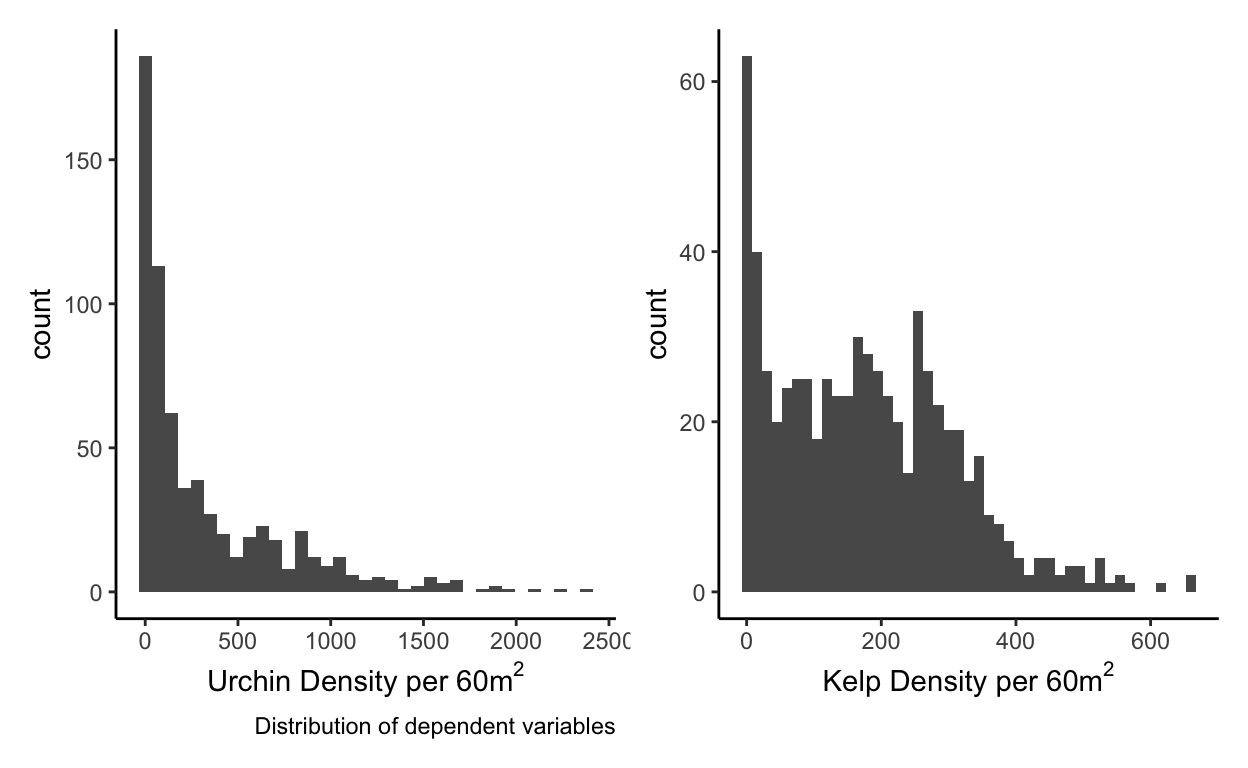
\includegraphics{mpasandkelp_files/figure-latex/unnamed-chunk-8-1.pdf}

\begin{Shaded}
\begin{Highlighting}[]
\NormalTok{caption }\OtherTok{=} 
\CommentTok{\# Log Transformed Normality }
\NormalTok{log\_urch\_dist }\OtherTok{\textless{}{-}} \FunctionTok{ggplot}\NormalTok{(}\AttributeTok{data =}\NormalTok{ annual\_mean) }\SpecialCharTok{+}
  \FunctionTok{geom\_histogram}\NormalTok{(}\FunctionTok{aes}\NormalTok{(log\_urch), }\AttributeTok{binwidth =} \FloatTok{0.15}\NormalTok{) }\SpecialCharTok{+}
  \FunctionTok{theme\_classic}\NormalTok{() }\SpecialCharTok{+}
  \FunctionTok{xlab}\NormalTok{(}\StringTok{"log Urchins"}\NormalTok{) }\SpecialCharTok{+}
    \FunctionTok{labs}\NormalTok{(}\AttributeTok{caption =} \StringTok{"Log transformed distribution of dependent variables"}\NormalTok{) }



\NormalTok{log\_mac\_dist }\OtherTok{\textless{}{-}} \FunctionTok{ggplot}\NormalTok{(}\AttributeTok{data =}\NormalTok{ annual\_mean) }\SpecialCharTok{+}
  \FunctionTok{geom\_histogram}\NormalTok{(}\FunctionTok{aes}\NormalTok{(log\_mac), }\AttributeTok{binwidth =} \FloatTok{0.15}\NormalTok{) }\SpecialCharTok{+}
  \FunctionTok{theme\_classic}\NormalTok{() }\SpecialCharTok{+}
  \FunctionTok{xlab}\NormalTok{(}\StringTok{"log Kelp"}\NormalTok{)}

\NormalTok{log\_urch\_dist }\SpecialCharTok{*}\NormalTok{ log\_mac\_dist}
\end{Highlighting}
\end{Shaded}

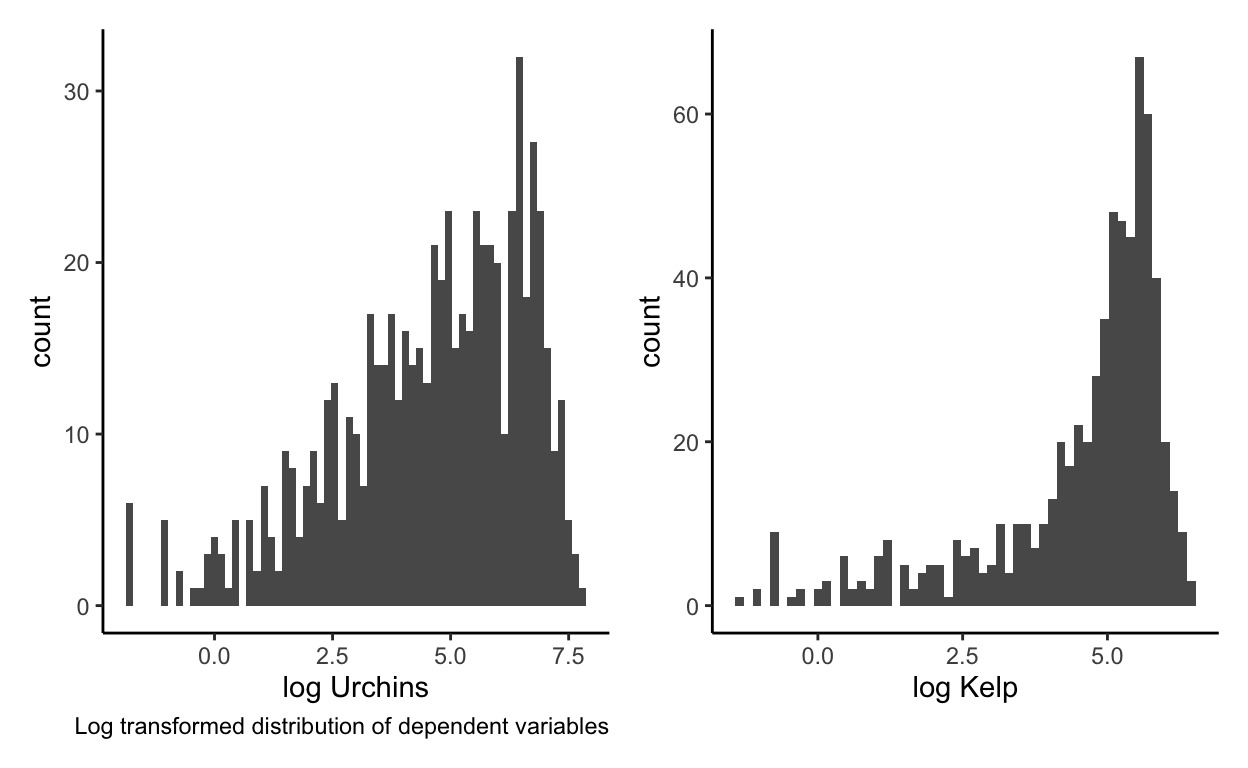
\includegraphics{mpasandkelp_files/figure-latex/unnamed-chunk-8-2.pdf}

\begin{Shaded}
\begin{Highlighting}[]
\CommentTok{\# Model Fit}

\NormalTok{aug }\OtherTok{\textless{}{-}}\NormalTok{ annual\_mean }\SpecialCharTok{\%\textgreater{}\%} 
  \FunctionTok{add\_predictions}\NormalTok{(mod) }\SpecialCharTok{\%\textgreater{}\%} 
  \FunctionTok{mutate}\NormalTok{(}\AttributeTok{residuals\_mac =}\NormalTok{ log\_mac }\SpecialCharTok{{-}}\NormalTok{ pred)}


\FunctionTok{ggplot}\NormalTok{(}\AttributeTok{data =}\NormalTok{ aug) }\SpecialCharTok{+}
  \FunctionTok{geom\_histogram}\NormalTok{(}\FunctionTok{aes}\NormalTok{(residuals\_mac), }\AttributeTok{binwidth =} \FloatTok{0.25}\NormalTok{) }\SpecialCharTok{+}
  \FunctionTok{theme\_classic}\NormalTok{() }\SpecialCharTok{+}
  \FunctionTok{xlab}\NormalTok{(}\StringTok{"Kelp Residuals"}\NormalTok{)}
\end{Highlighting}
\end{Shaded}

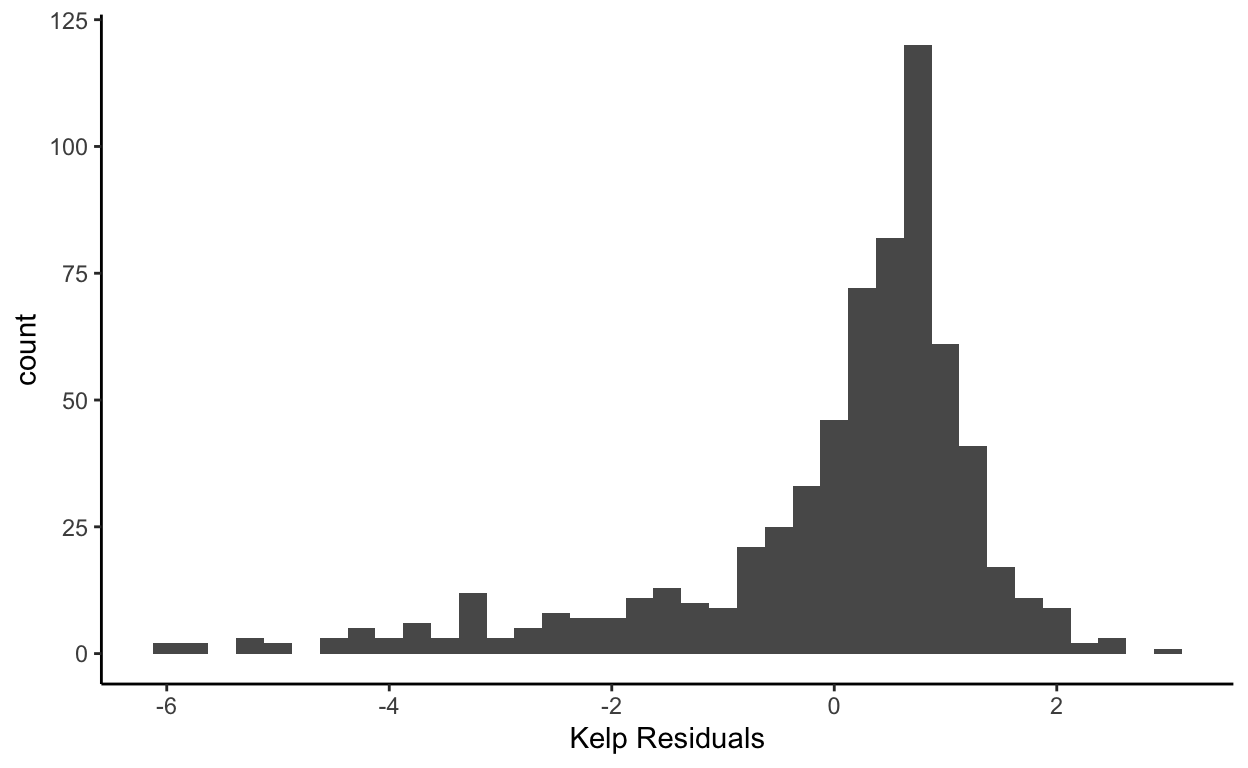
\includegraphics{mpasandkelp_files/figure-latex/unnamed-chunk-8-3.pdf}

\begin{Shaded}
\begin{Highlighting}[]
\FunctionTok{qqPlot}\NormalTok{(aug}\SpecialCharTok{$}\NormalTok{residuals\_mac) }
\end{Highlighting}
\end{Shaded}

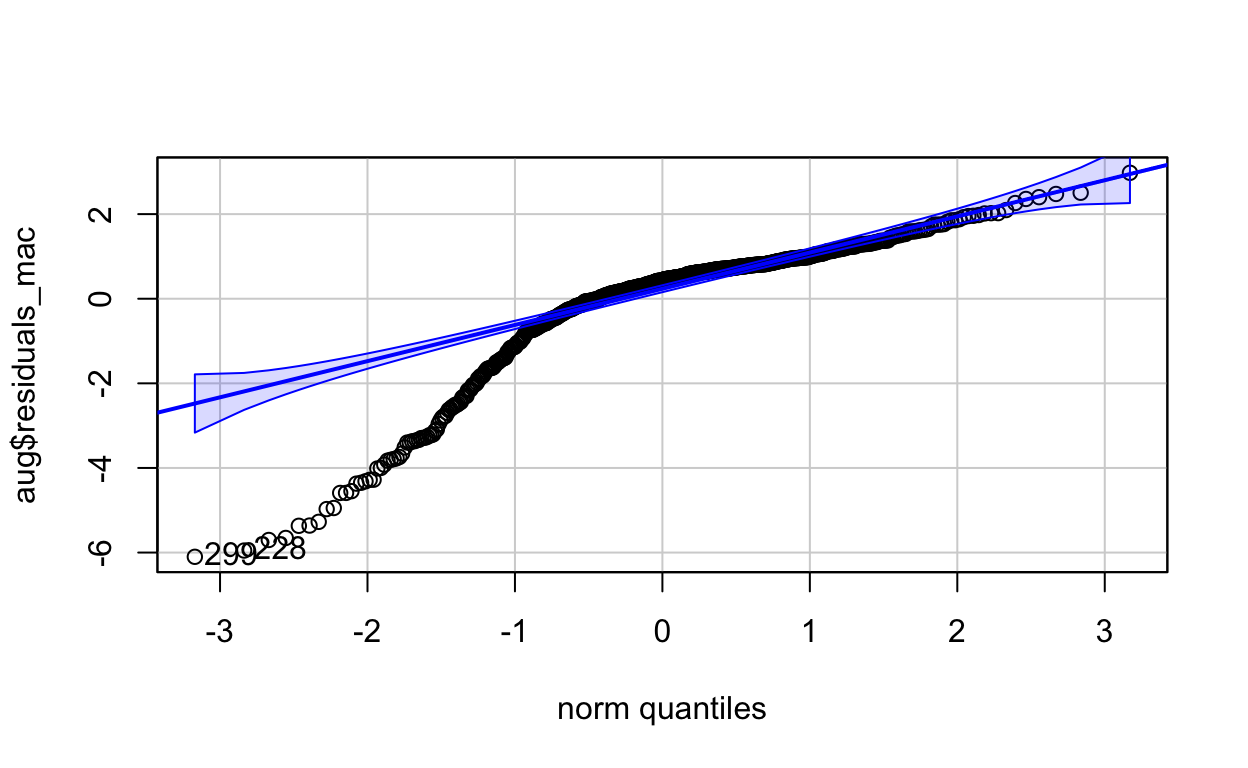
\includegraphics{mpasandkelp_files/figure-latex/unnamed-chunk-8-4.pdf}

\begin{verbatim}
## [1] 299 228
\end{verbatim}

\begin{Shaded}
\begin{Highlighting}[]
\FunctionTok{paste0}\NormalTok{(}\StringTok{"mean residuals "}\NormalTok{, }\FunctionTok{mean}\NormalTok{(aug}\SpecialCharTok{$}\NormalTok{residuals\_mac))}
\end{Highlighting}
\end{Shaded}

\begin{verbatim}
## [1] "mean residuals -2.19943444182886e-15"
\end{verbatim}

\begin{Shaded}
\begin{Highlighting}[]
\FunctionTok{ggplot}\NormalTok{(}\AttributeTok{data =}\NormalTok{ aug) }\SpecialCharTok{+}
  \FunctionTok{geom\_point}\NormalTok{(}\FunctionTok{aes}\NormalTok{(}\AttributeTok{y =}\NormalTok{ residuals\_mac, }\AttributeTok{x =}\NormalTok{ den\_STRPURAD), }\AttributeTok{alpha =} \FloatTok{0.3}\NormalTok{) }\SpecialCharTok{+}
  \FunctionTok{geom\_hline}\NormalTok{(}\AttributeTok{yintercept =} \DecValTok{0}\NormalTok{, }\AttributeTok{linetype =} \StringTok{"dashed"}\NormalTok{) }\SpecialCharTok{+}
  \FunctionTok{theme\_classic}\NormalTok{() }\SpecialCharTok{+}
  \FunctionTok{xlab}\NormalTok{(}\FunctionTok{expression}\NormalTok{(}\StringTok{"Urchin Density per 60m"}\SpecialCharTok{\^{}}\DecValTok{2}\NormalTok{)) }\SpecialCharTok{+}
  \FunctionTok{ylab}\NormalTok{(}\StringTok{"Kelp Residuals"}\NormalTok{)}
\end{Highlighting}
\end{Shaded}

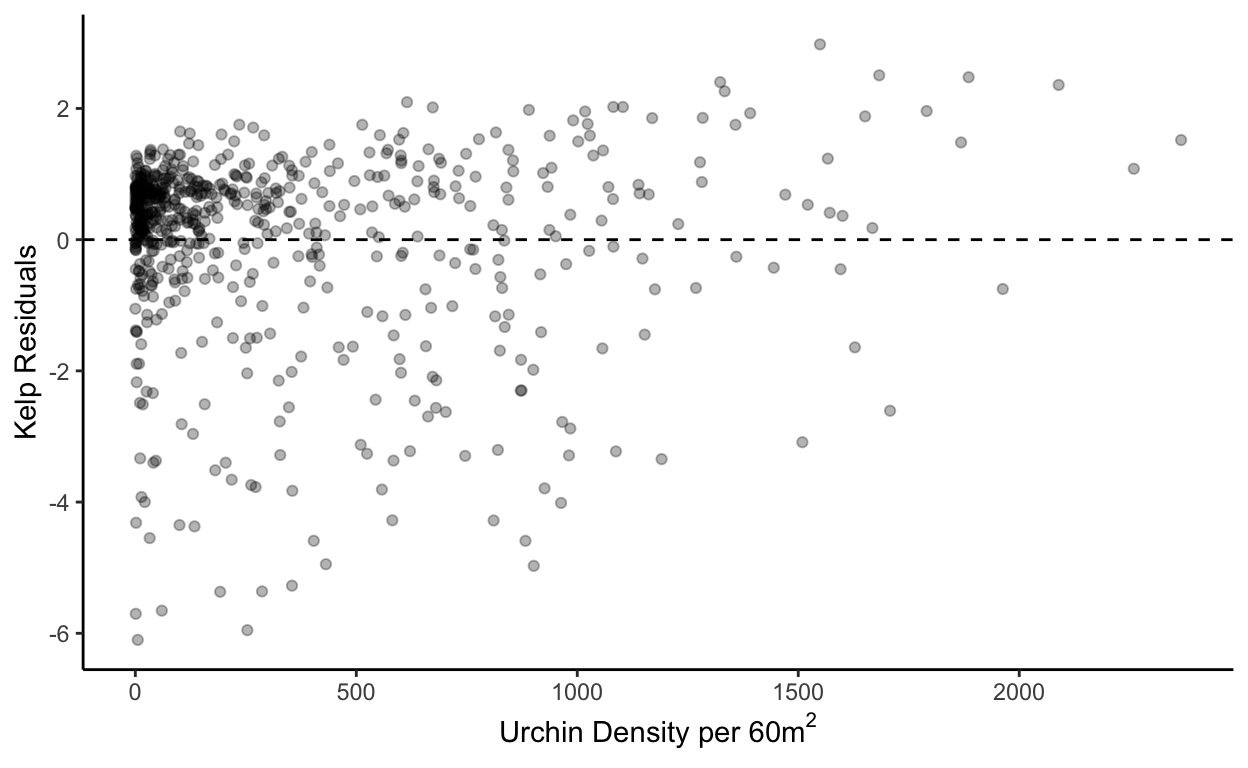
\includegraphics{mpasandkelp_files/figure-latex/unnamed-chunk-8-5.pdf}

\end{document}
